%%---------------Chapter 5------------------------------
% \documentclass[../UNBThesis2.tex]{subfiles}
\setlength{\parindent}{2em}
% \usepackage{caption}
% \usepackage{subcaption}
% \usepackage{floatrow}
% \usepackage[label font=bf,labelformat=simple]{subfig}
% \floatsetup[figure]{style=plain,subcapbesideposition=botton}

%itemize without indent :\setlength{\itemindent}{-1.5em}
%single paragraph indent --> /noindent

%short term memory

\definecolor{dkgreen}{rgb}{0,0.6,0}
\definecolor{gray}{rgb}{0.5,0.5,0.5}
\definecolor{mauve}{rgb}{0.58,0,0.82}

\lstset{frame=tb,
  language=Python,
  aboveskip=3mm,
  belowskip=3mm,
  showstringspaces=false,
  columns=flexible,
  basicstyle={\small\ttfamily},
  numbers=none,
  numberstyle=\tiny\color{gray},
  keywordstyle=\color{blue},
  commentstyle=\color{dkgreen},
  stringstyle=\color{mauve},
  breaklines=true,
  breakatwhitespace=true,
  tabsize=3
}






% \begin{document}

\chapter{Implementation}

In this Chapter, the design and implementation of the DSAP algorithm are described. Next, two experiments are presented that are related to applying the proposed DSAP model to find stair usage patterns and occupant behaviour in indoor spaces. 

%The two studies are: an e-counter based Indoor staircase usage experiment and a WiFi fingerprint-based Indoor Localization dataset. 


%The DSAP algorithm is a clustering approach consisting of phases as shown in Figure \ref{frame}. The online micro-cluster phase detects newly arriving data points and updates the clusters. The offline macro-cluster phase generates summary clusters periodically or at the end of the stream. The intrinsic clustering validation Phase ,and clustering performance evaluation phase assesses the clustering quality based on different criteria. The last phase, comparison between DSAP and streaming K-means shows the DSAP results compare to the streaming K-means results.






%\section{DSAP Clustering Algorithm}
%The Data Stream Affinity Propagation (DSAP) algorithm is an online and offline algorithm that generates micro and macro clusters based on a landmark time window model. This section describes the DSAP algorithm, which extends the AP algorithm for streaming data clustering applications. 

%Considering the challenges of clustering data streams to have updated clusters, this algorithm generates a model that describes the data streams and incrementally updates the model to generate recent clusters with any type of data. The DSAP algorithm consists of two phases: online phase and offline phase. these two phases receive and analyze data streams in real-time. However, the two datasets that are analyzed in this work were obtained from experiments performed over a fixed time period. For this reason, we had to convert the data into a simulated data streams, we discuss about this approach in the next section.

\section{Data Stream Simulation}
%Data elements in the stream arrive online, there is no control over the order in which elements arrive, either within a single stream. Streams are potentially unlimited in size

% #####################################
%  Using affinity propagation for streaming clustering faces two difficulties. First, AP has been implemented for batch processing but it should handle data clustering and large datasets in the online mode. The most important point to consider is AP suffers from quadratic computational complexity.
% Extensive data that are continuously coming are required to store. Analyzing big datasets and extracting patterns is not possible with affinity propagation due to the time complexity issue.
% One way to apply affinity propagation algorithm is using the divide and conquer approach \cite{khalilian2016data}. This approach introduced by Nittel et al.\cite{nittel2004scaling}, has mainly three steps as shown in Figure \ref{dividee}: partitioning the dataset into different chunks, then clustering each chunk and find the results, lastly, computes the results out of all chunks of data. 

% \begin{figure}[!h]
%     \centering
%     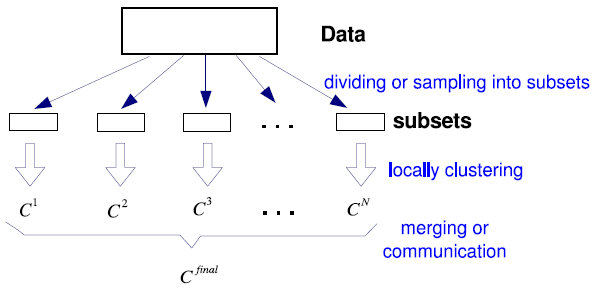
\includegraphics[width = 11 cm]{image/Chapters/Chapter3/divide.PNG}
%     \caption{Divide and conquer approach to generate clustering out of big data \protect\cite{zhang2009toward}}
%     \label{dividee}
% \end{figure}


% Our first attempt working with the extensive dataset was to implement this technique to generate data stream clustering \cite{ivarispatio}, and it was the first version of DSAP, which is presented in this thesis. However, it has a history of all data points, and the time and memory complexity are still high, and most algorithms that have this approach are unable to track the change in the trend of the data stream. 
% Due to the reason above, some research has been done on AP streaming clustering and introduce new approaches.

%##################################################### MOnica

In order to mimic a data stream, it was necessary to convert the collected data into a stream. For DSAP, this conversion was performed using the scikit-multiflow data stream simulation framework from Python.  Scikit-multiflow is a free and open-source tool and it is part of the River machine learning library in Python \cite{montiel2018scikit}. The prerequisites to install scikit-multiflow package (\textit{skmultiflow}) are NumPy and Cython libraries. 

The \texttt{skmultiflow.data} module includes two group of classes that either perform batch-to-stream conversions or generate standard data streams like waveform, Gaussian as shown in Figure \ref{sci}. The batch-to-stream conversion classes generates streams from a file source (.csv files) in the disk or from data in the memory.

\begin{figure}[!ht]
    \centering
    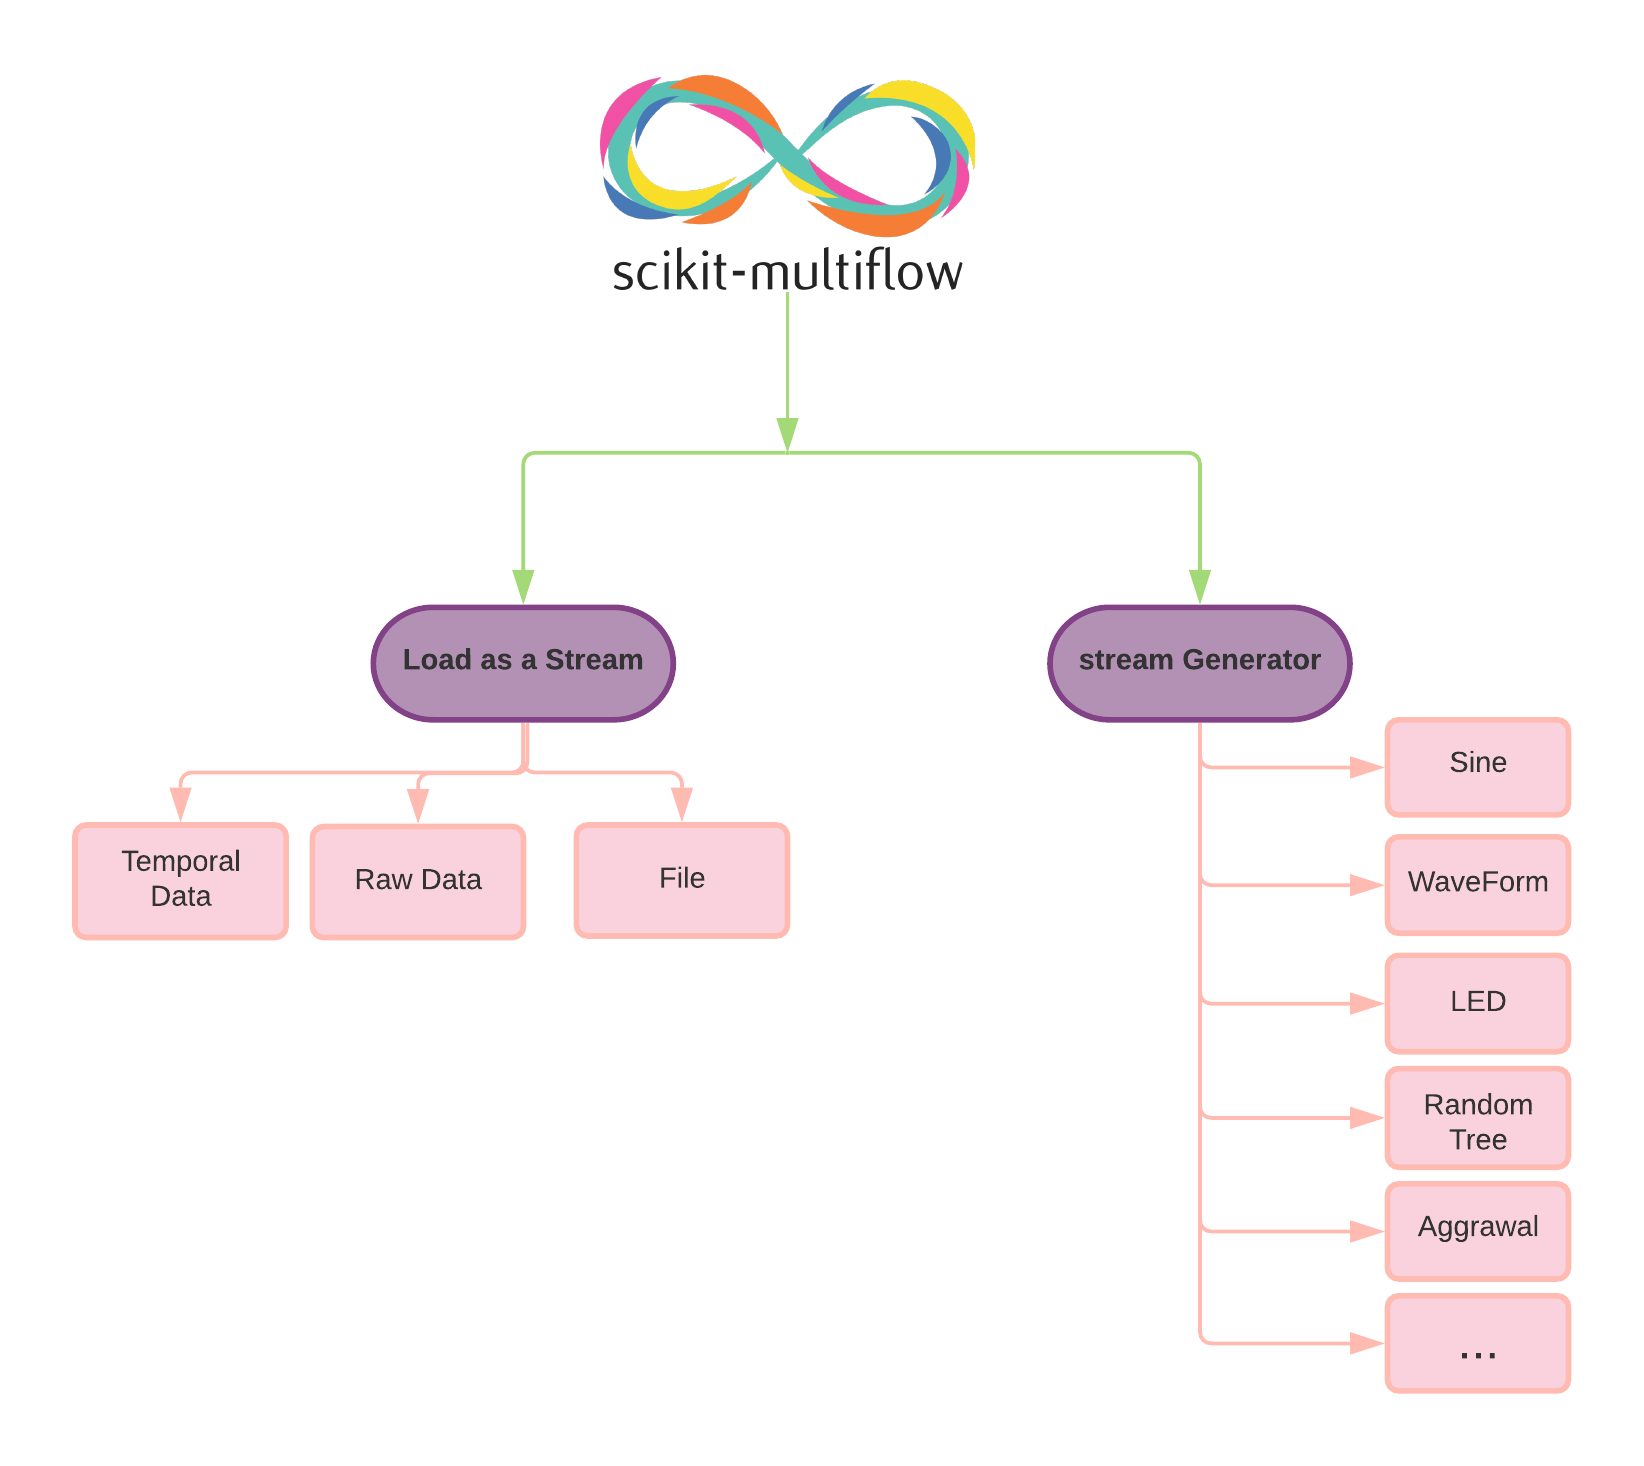
\includegraphics[width = 11 cm]{image/Chapters/Chapter5/multiflow.png}
    \caption{The scikit-multiflow data stream generator modules: load as a stream and stream generator}
    \label{sci}
    \end{figure}

The DSAP uses the \textit{skmultiflow.data.FileStream} class for generating data stream from any CSV file. It is part of the \texttt{skmultiflow.data} module and imported as: \texttt{skmultiflow.data.file\_stream}. Then, the data set is loaded as a stream (\texttt{ stream = FileStream (filepath)}), which is generated by the FileStream class. The Stream class is in charge of providing data inside scikit-multiflow and it runs upon request a number of samples, in a way such that old samples cannot be accessed at a later time. 

The most important method of the stream class is \texttt{next\_sample()}, which returns the next window at the start of every time interval. Also, the function \texttt{has\_more\_samples()} checks if any data point is left in the data set for consideration. Even though these packages are very capable of mimicking the data observed in data stream, the user still must acknowledge the limitations of such techniques. The difference from the real data stream can result from many potential shortcomings of the stream simulation models. The stream simulation packages do not have the support for generating realistic latency information, missing data, mixed timestamps, varying data cadence, and others. Hence any evaluation of the robustness and efficacy of a stream clustering algorithm done using the simulated streams should be cautiously accepted. 


\section{DSAP Clustering Phase}
%This section describes how the DSAP algorithm is implemented for data stream clustering using the landmark time window model in Python programming language. 

The DSAP source code in Python programming language has been made freely available at: \url{https://github.com/nasrineshraghi/DSAP}. The detailed description of each section of the code is presented below.

After the conversion of the CSV file data to a simulated stream, a landmark time window function \texttt{getWindowSize(start\_time, L)} is applied on the data points. This function finds the number of data points in a particular time window and returns this value. 

\begin{lstlisting}
# Estimate the number of data points within a time window
def getWindowSize(start_time,L):
    try:
        idx1 = np.where(df[:,2] >= start_time )[0][0]
        idx2 = np.where(df[:,2] >= start_time + L )[0][0] 
    except:
        idx1 = 0
        idx2 = 0
    XOmega = idx2 - idx1
# XOmega is window size
    windowSize = XOmega
    return windowSize
\end{lstlisting}


Every time window has a different start time, and this start time should be updated after the end of the window length is reached (\texttt{start\_time = start\_time + L}). If there is no data point available in a particular window or the number of them are few, the scikit-multiflow function (\texttt{stream.next\_sample(windowSize)}) skips that window and goes to the next one.

\begin{lstlisting}
from skmultiflow.data.file_stream import FileStream
# skip if the window is empty or few number of points are available
# For example 5 data points or less 
        if windowSize < 5:
            X = stream.next_sample()
            continue
        else:    
            j = j +1
\end{lstlisting}


It should be noted that if the landmark window is a count-based window instead of time, \texttt{windowSize} needs to be defined as the number of data point in each window instead of getting the value from the \texttt{getWindowSize} function above. For instance \texttt{windowSize = 100} means that each time the latest 100 data point from the stream are accessed. In this case number of data points in the window $\Omega$ is equal to $L$.

The DSAP online micro-cluster phase is implemented in three steps as described before in Chapter 4: initialization, comparison, and ActivateAP with update $\epsilon_{W_j}$.

In the Initialization step, the AP algorithm is applied on all data points present in the first window $W_0$ from the data stream. % (\texttt{AffinityPropagation().fit($W_0$)})

\begin{lstlisting}
#(1) Initialization. AP on the first time window
from sklearn.cluster import AffinityPropagation 
# AP library needs to be added first
preference = np.median(euclidean_distances(W0, squared=True))
AP = AffinityPropagation(preference, damping).fit(W0)
cluster_centers_indices = AP.cluster_centers_indices_
labels = AP.labels_
Cm = AP.cluster_centers_
n_clusters_ = len(cluster_centers_indices)
X = np.array(xi)
X_label = np.array(labels)
\end{lstlisting}

The AP algorithm generates a set of micro clusters ($C{_m}$). To initiate the DSAP model, a sufficient number of data points is required in the first window. Hence, it is important to choose an optimal value for the window size; otherwise, DSAP cannot reach convergence, and the model will fail. After the micro-clusters are generated, the distance matrix of all data points and centroids in each cluster are calculated by the \texttt{getAdaptiveThreshold()} function. The average distance of these values gives the initial $\epsilon_{W_0}$ that will be used in the comparison step.


\begin{lstlisting}
from scipy.spatial import distance
# Calculate the threshold distance
def getAdaptiveThreshold(Wj,Cm):
    epsilon = np.mean(distance.cdist(Wj,Cm,'Euclidean'))
    return epsilon 
\end{lstlisting}

In addition, the timestamp associated to each cluster centroids should be kept in an array with the size of initial centroids. The time for all centroids in the first window are equal.

\begin{lstlisting}
#time associated to initial centroids
tq = np.ones(len(Cm))*start_time
tq = tq.astype(int)
\end{lstlisting}


The output of the initialization step are a set of micro-clusters with centroids ($C_m$) and an initial threshold value ($\epsilon_{W_0}$).

The next step of the online micro-cluster phase is comparison. For the following windows from $W_1$ to $W_N$, all data points in each window are compared with the existing micro-clusters. The Euclidean distance of each new point $x_i$ in the window to its closest micro-cluster centroid is calculated. If the distance is less than the threshold $\epsilon_{W_j}$, $x_i$ is added to the micro-clusters and the timestamp associated to those specific centroids needs to be updated. Otherwise, it is kept temporarily in the time-window repository until all data points in the window are being evaluated. 

\begin{lstlisting}
#(2) Comparison step.
# Update the start time for each window
windowsize = getWindowSize(start_time, L)
start_time = start_time + L
indx = 0
repository = []
for i in range(windowSize):
    d = distance.cdist(Cm,x,'Euclidean')
    ind = np.argmin(d)    
    if min(d) < epsilon:
         X = np.concatenate((X , np.reshape(x[i,:],(-1,2))))
         X_label = np.concatenate((X_label , np.reshape(ind,(-1))))
         #Updating time associated to centroid met in this step
         tq[ind] = start_time
    else:
        repository.append(x[i])       
        indx = indx +1
\end{lstlisting}

%At the end, the AP will apply again to find new micro-clusters out of these data. If there is no data point is in the cache, the next window will come in the model.

In the next ActivateAP step, AP is applied on all the remaining data points in the time-window repository whose distance from the centroids are more than the adaptive threshold $\epsilon_{W_j}$ for the current time window. In the end, clusters obtained from this step are added to the updated micro-clusters.  


\begin{lstlisting}
#(3) ActivateAP step for the time-window repository points
repositorydata = np.array(repository)
preference = np.median(euclidean_distances(repositorydata, squared=True))
AP_crepository = AffinityPropagation(preference, damping).fit(crepositorydata)
C`m = AP_repository.cluster_centers_
AP_repository_label = AP_repository.labels_
X = np.concatenate((X , np.reshape(repositorydata[i,:],(-1,2))))
X_label = np.concatenate((X_label , np.reshape(AP_repository_label,(-1))))
#C`m is the Cm prime, new micro-clusters
Cm = np.append(C`m, Cm, axis = 0)
# Assign timestamp to new micro-clusters
repository_tq = np.ones(len(C`m))*start_time
repository_tq = repository_tq.astype(int)
tq = np.concatenate((tq, repository_tq), axis=0)
\end{lstlisting}


As new micro-clusters are generated at the end of the ActivateAP step, the threshold value needs to be recalculated based on the updated micro-clusters. Once again the adaptive threshold function is called upon to estimate new threshold values. This value is compared with the threshold $\epsilon_{W_j}$. If the value is greater than $\epsilon_{W_j}$ then a average of the two thresholds is selected as the new threshold otherwise the threshold remains unchanged. The decision to choose the average of the two numbers was taken to ensure that the threshold does not blow up in size due to a sparse cluster or noise.
\begin{lstlisting}
# Update the threshold value.
epsilonC`m = getAdaptiveThreshold(C`m, repositorydata)
if epsilon < epsilonC`m:
    epsilon = (epsilonC`m + epsilon)/2  
\end{lstlisting}

In order to keep the number of micro-clusters under control and avoid obsolete clusters, cluster centroids that are older than the expiration number $e_x$ times the time period (older than a specific number of landmark) are removed periodically. The oldest relevant time is calculated by subtracting the $e_x$ number of time periods from the current timestamp (\texttt{start\_time}). The centroids with timestamps greater than this value are retained in the updated centroids along with their updated associated timestamps. Based on the duration of interest this expiration value is set by the user at the start of the stream clustering process. 



\begin{lstlisting}
# Remove old micro-clusters
# Number is an integer value defines by the user
ex = int Number
remain_centers = np.ones(len(tq))
for i in range(len(tq)):
    # Remove the centroids with time more than the ex
    if tq[i] < start_time - ex * L:
        remain_centers[i] = 0
indx_remain= np.where(remain_centers==0) 
Cm  = Cm[remain_centers==1]
tq = tq[remain_centers==1]
a = indx_remain[0]
for j in range(len(a)):
    indx = np.where(X_label == a[j])
    # Remove the labels with time more than ex
    X_label= np.delete(X_label, indx)

\end{lstlisting}


The next phase of the DSAP algorithm is the offline macro-cluster phase which generates final clusters by applying the AP algorithm one more time to all the micro-cluster centroids accumulated during the online phase (\texttt{AffinityPropagation().fit ($Cm$)}). In the offline phase only the summary statistics represented by the micro-clusters centroids stored during the online phase is used and not the actual data set itself. The number of micro-clusters is a lot smaller than the total number of points in the data set that it represents. The number of macro-clusters obtained in this phase are less than the number of micro-clusters as they summarize the whole period of observation and not individual windows. The pseudo-code presented in Algorithm \ref{algSDAPi} shows the outline of the entire DSAP algorithm. 

\begin{lstlisting}
# Offline Macro-clustering Phase
preference = np.median(euclidean_distances(Cm, squared=True))
AP_mac = AffinityPropagation(preference, damping).fit(Cm)
cluster_centers_indices_mac = AP_mac.cluster_centers_indices_
cluster_centers_mac = AP_mac.cluster_centers_
mac_label = AP_mac.labels_

\end{lstlisting}


%\todo[inline]{ALGORITM HERE} 
%%%%%%%%%%%%%%%%%%%%% DSAP  %%%%%%%%%%%%%%%%%%%%%%%%%%%%%%%%%%

\begin{algorithm}[htbp]
       
\caption{DSAP Algorithm}
    \label{algSDAPi}
\small
    \textbf{Input:}
         Data stream: $S$ as windows ${ W_0,W_1, ..., W_N : W_j = x_1, ..., x_{\Omega}}$ with the length L, ex ;\newline 
    \textbf{Hyperparameters:}
        {Preference, Damping, $\epsilon_{W_j}$}\newline
        \textbf{Output:}
        Set of micro clusters with centroids $Cm= [Cm_1,Cm_2, ..., Cm_q]$,  set of macro clusters with centroids $C_M= [C_{M_1}, C_{M_2}, ...C_{M_k}]$ \\
        
        \SetKwFunction{FIROC}{getWindowSize} 
         \SetKwProg{Fn}{Function}{}{}
         \Fn{\FIROC{$start\_time, L$} 
         }{
         $time\_period = start\_time + L$ \\
         $windowSize$ = $S(time\_period)$
        %  $windowSize = time\_period - start\_time$
         }
         \KwResult{$windowSize$} 
                 \SetKwFunction{FIROC}{getAdaptiveThreshold}          
         \SetKwProg{Fn}{Function}{}{}
         \Fn{\FIROC{$W_j$, $Cm$}}{
         $\epsilon_{W_j}$ = mean(d($W_j, Cm$))
                  }
         \KwResult{$\epsilon_{W_j}$} 
        %  \Statex  \hfill              
         \ContinuedFloat\hfill
        \textcolor{red}{\textbf{Online Phase}}\\
         j = 0\\
         \While{!(stream.has\_more\_samples())}{
         
      	\eIf{(j == 1) %\tcp{\color{green}First window}
       	} 
       	{\hfill \Comment{Initialization}\\
       	$W_0$ = \texttt{S.getWindowSize($start\_time, L$)}\newline
       	\SetKwFunction{FIROC}{AP}          
             \SetKwProg{Fn}{Function}{}{}
             \Fn{\FIROC{ $W_0$}}{}
             \KwResult{Initial micro-clusters: $Cm = [Cm_1,Cm_2,...,Cmq]$, label data points: $X$, $[tq] = start\_time$}\\
             $\epsilon_{W_j}$ = getAdaptiveThreshold($W_0, Cm$)\;
            
             }
             {
      $W_j$ = \texttt{S.getWindowSize($start\_time + L*j, L$)}\\
      $start\_time = start\_time + L$\\
       
              %  \If{getWindowSize == 0}
      %  {$W_j = W_j + 1$}  \newline
        % \newline
        
         %\Statex \hfill     \textbf{{Online Phase:}}\\
        \For{($x_i:i = 1:\Omega$)}{\hfill \Comment{Comparison}\\
        $[d]$ = d($[Cm], x_i$) \newline
        
        \eIf{min ($[d]) < \epsilon_{W_j}$}
        {   
        $Cm[X] \leftarrow{x_i}   $
        (merge with micro\_clusters)\\
        $[tq] = start\_time$
        
        }
        {
        $repository \leftarrow{x_i} $ 
        
        %\STATE $W_i \xrightarrow \mathrm{C_{m0}}$\;
        }
        
        \hfill \Comment{ActivateAP}\\
        %if 1st
        %  \If{$i == \Omega$}
        %  {                                  
         \SetKwFunction{FIROC}{AP}          
         \SetKwProg{Fn}{Function}{}{}
         \Fn{\FIROC{repository}}{}
         \KwResult{new micro-clusters:$[C'm]$\\
                $\epsilon_{W_J}'$ = getAdaptiveThreshold($C'm,repository$)\\
                $tq_{repository} = start\_time$
                }

        %  }
        }

        Update micro\_clusters: $Cm = Cm + C'm$ \\
        Updated timestamp $tq = tq + tq_{repository}$\\
        Update Threshold : $\epsilon_{W_j}$
        
        

      }
       
      \If{$tq < start\_time - ex * L$}
        {Discard Cm }
         
        \textbf{Results: } Micro Clusters: $Cm= [Cm_1,Cm_2,Cm_3, ..., Cm_q]$ %}
        }
        \end{algorithm}
        \begin{algorithm}
          \small
         \If{end of S}{                        
          \ContinuedFloat\hfill
\textcolor{red}{\textbf{Offline Phase}}\\
         
         \SetKwFunction{FIROC}{AP}
         \SetKwProg{Fn}{Function}{:}{}
        \Fn{\FIROC{$Cm$}}{}
     \KwResult{Macro Clusters: $C_M= [C_{M_1}, C_{M_2}, ...C_{M_k}]$} 
     }

\end{algorithm}


%\section{Streaming K-means Algorithm}
% The established streaming K-means algorithm was chosen for comparison with the proposed DSAP algorithm. The variant of the algorithm for this study is part of the stream framework implemented in R programming language for data stream modeling and associated data mining tasks such as clustering and classification \cite{packager}. This version of the streaming K-means algorithm was chosen as the stream package not only provides an easy interface for k-means cluster computation, but also includes a lot of other popular clustering techniques that will aid in future model comparisons. Streaming-Kmeans has been successfully used to analyze data streams from wearable devices by our group at UNB using the same R package. 

% The R stream framework consists of two main components as shown in Figure \ref{streammm}:
% \begin{itemize}
%     \item Data Stream Data (DSD) object simulates the data stream.
%     \item Data Stream Clustering (DSC) task to find clusters out of a simulated data stream.
% \end{itemize}

% \begin{figure}[!h]
%     \centering
%     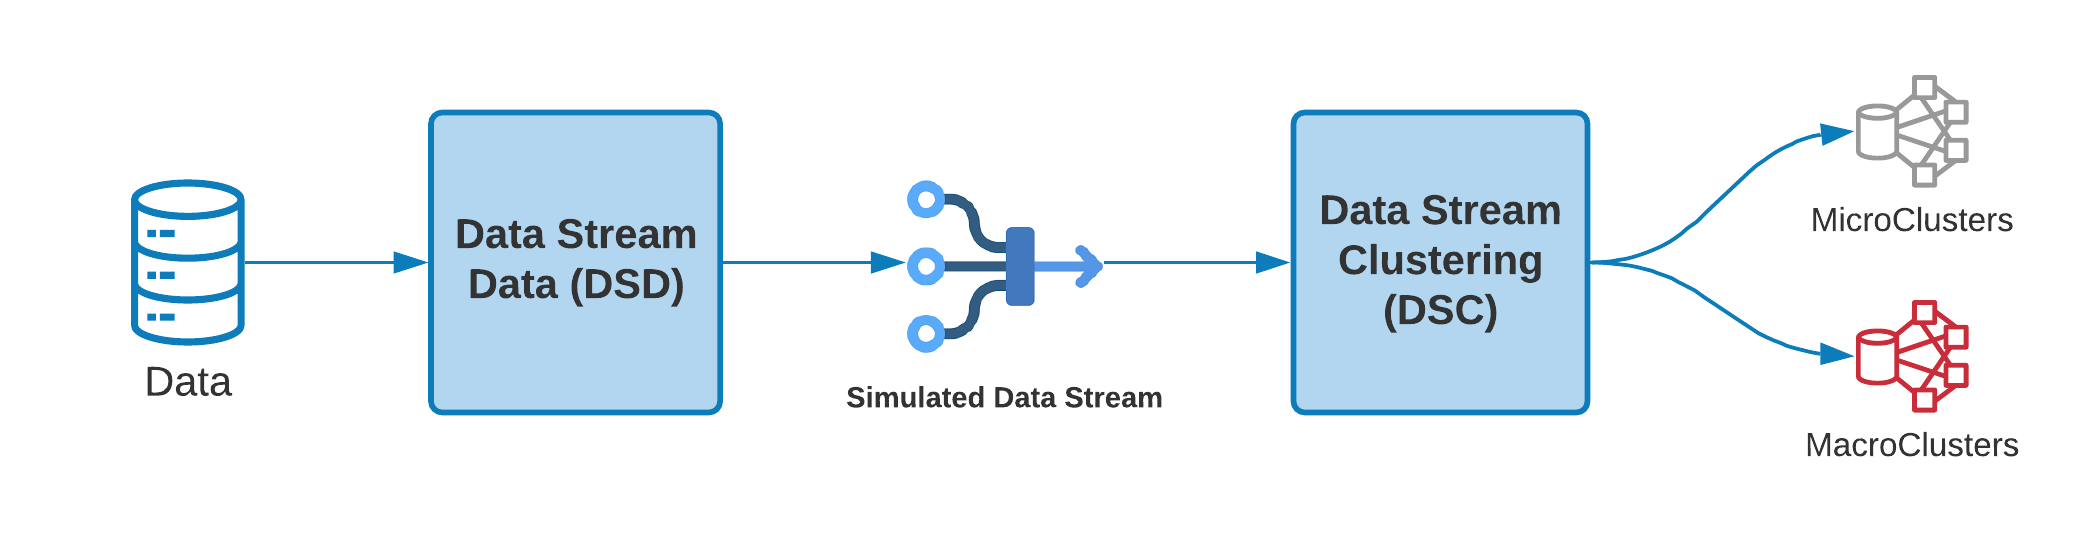
\includegraphics[width=.9\textwidth]{image/Chapters/Chapter5/RKmeans.png}
%     \caption{ Data stream simulation with R stream framework. This part is called DSD, has tree modules.}
%     \label{streammm}
% \end{figure}




% % Overview of R framework for streaming K-means with two steps: the data stream Data (DSD) and data stream clustering (DSC) class structure.    
    
% \subsection{Data Stream Simulation}
% %  All these modules are presented in the \texttt{Stream} package.
% The Data Stream Data (DSD) object which is part of the \texttt{Stream} package is an abstraction layer that connects to any streaming data source. The stream package provides several DSD implementations as shown in Figure \ref{dsd}. The simulated stream generated by the DSD can mimic static streams as well as streams with concept drift. In-flight implementation can be used to standardize in terms of centering and scaling data in a data stream. % in-flight.  
% Read data connector class provides simulated streams in three different ways: \texttt{DSD\_Memory}, gives streaming interface to data in memory which represents a part of data, \texttt{DSD\_ReadDB} provides an interface from SQL query to the database, and \texttt{DSD\_ReadCSV} reads data line by line from a file or a connection and makes it available in a streaming manner. This enables a system to process data that is larger than the available memory. Connections to real data can be applied to read from real-time data streams.

% \begin{figure}[!htb]
%     \centering
%     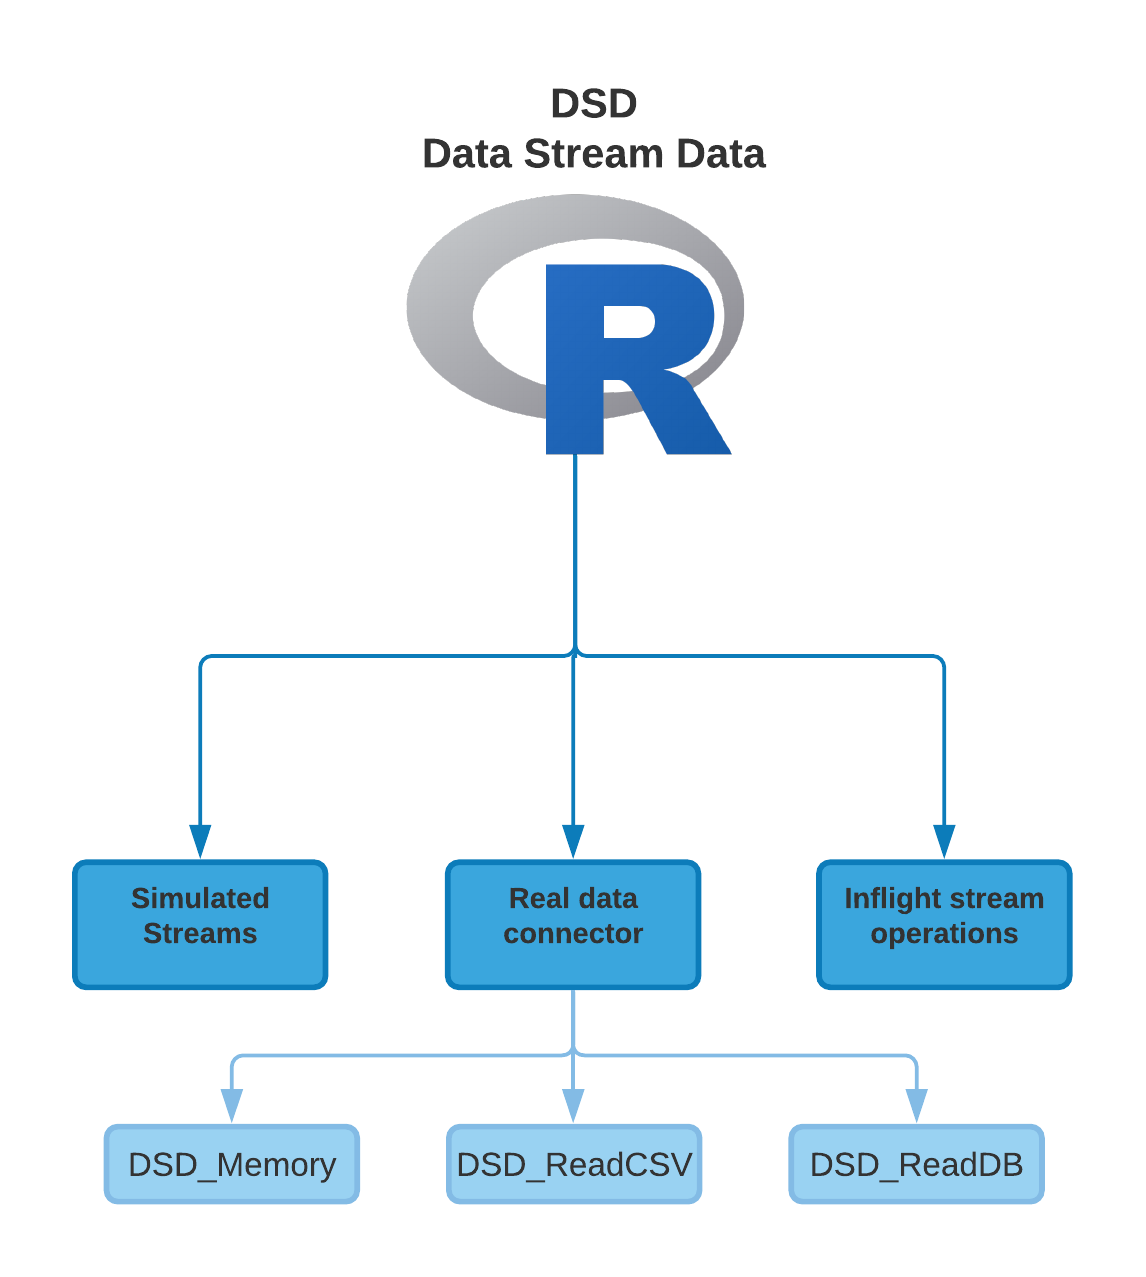
\includegraphics[width = 8 cm]{image/Chapters/Chapter5/dsd.png}
%     \caption{ .}
%     \label{dsd}
% \end{figure}


% To generate data stream out of the CSV files, \texttt{DSD\_ReadCSV()} class is used. This class has some unique features such as the ability to change position in the file and reset it to the beginning and the connection can be closed anytime. All the DSD packages have the same interface using the two functions: a creator function whose outcome is not a dataset but an object describing the stream's properties and its current state, and a data generating function like \texttt{get\_point()} that is handled to get the next data point from the stream.

% % \begin{lstlisting}
% #reading the data out of file
% stream <- DSD_ReadCSV(file, loop=FALSE, sep=",", header=FALSE, ...)
% \end{lstlisting}

% \subsection{Data Stream Clustering}
% After applying a DSD class to generate the data stream, the next step is to analyze the data stream to generate clusters. The Data Stream Clustering (DSC) object in the stream package provides multiple options to analyze the data as shown in Figure \ref{dsc}. The two stage \texttt{DSC\_TwoStage} clustering framework was chosen for this study. It combines two abstract classes that create micro-clusters \texttt{DSC\_Micro} and macro-clusters\texttt{DSC\_Macro}.
% % \begin{lstlisting}
% # create a clustering process that uses a window for the online and k-means for the offline phase 
% win_km <- DSC_TwoStage(
%   micro = DSC_Window(horizon, lambda),
%   macro = DSC_Kmeans(k)
%   )
% win_km
% update(win_km, stream, 200)
% \end{lstlisting}
% As shown in the above code, the 
% The two classes in \texttt{DSC\_TwoStage} which form the core of the streaming K-means clustering algorithm are: 

%     \begin{itemize}
%         \item\texttt{DSC\_Window():} provides a clustering interface to the data stream operator. It implements a window model, which keeps a specified number of data points from the stream in a format defined by the user. This number is the window length. 
        
%         \item\texttt{DSC\_Kmeans():} class implements the R version of the k-means algorithm for reclustering a set of micro-clusters. In this version of k-means the data points (micro-clusters) can be weighted based on the micro cluster density. The streaming k-means clustering algorithm requires a continuously updated set of micro clusters.

%     \end{itemize}


% This algorithm is capable of handling data as sliding or damped time windows that are generated by the \texttt{DSC\_Window()} class. For the sliding time window a user-specified number (window length) of the most recent data points of the stream are kept as the micro-cluster. For the damped window model, data points in the window have a weight that deceases exponentially with age. \texttt{DSC\_Window()} can also generate and analyze hopping/landmark time window model as this is just a special case of the sliding time window when there is no overlap in sliding window. In the macro-cluster step the K-means algorithm needs to be provided with the number of clusters parameter $k$. This parameter is set by applying elbow method that was discussed earlier in section \ref{kmeansalgo}. Ideally this parameter should be automatically estimated but due to the small datasets analyzed for this study this wasn't deemed necessary and hence the $k$ value was calculated separately.

% \begin{figure}[]
%     \centering
%     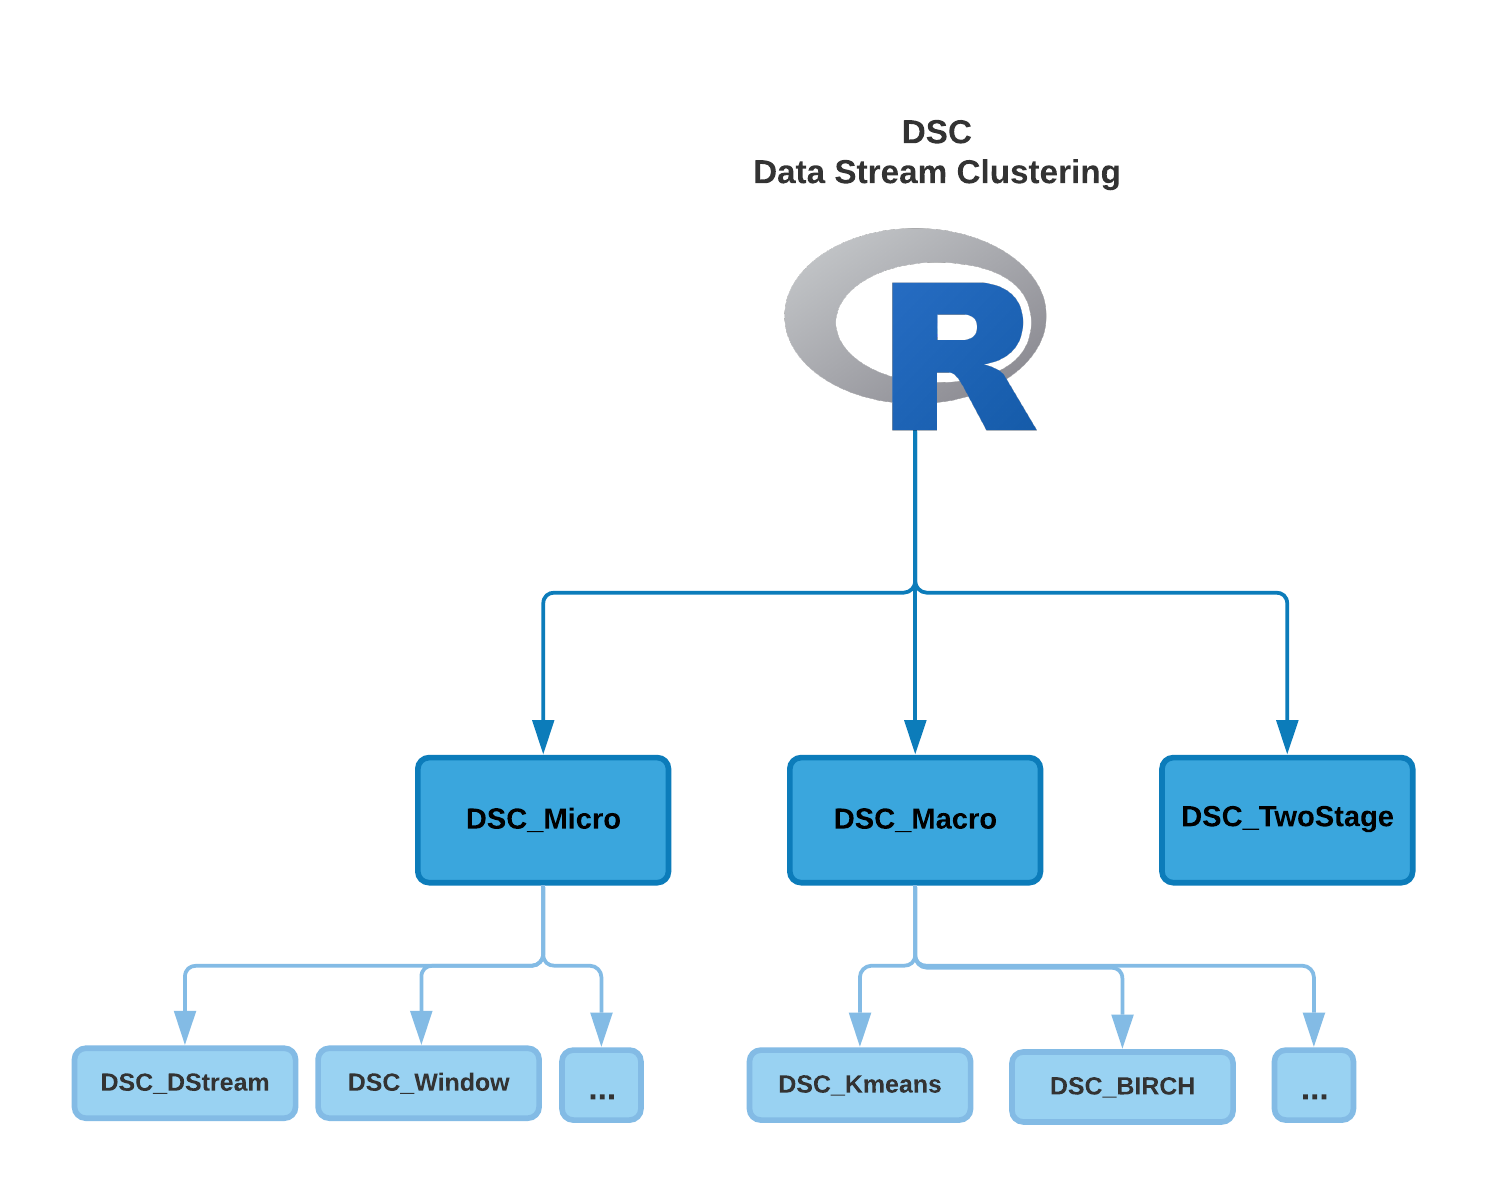
\includegraphics[width=.7\textwidth]{image/Chapters/Chapter5/DSC_all.png}
%     \caption{ .}
%     \label{dsc}
% \end{figure}



\section{Intrinsic Clustering Validation Phase}
To validate the clustering results, three Intrinsic evaluation metrics: Silhouette Coefficient, Caliński-Harabasz Index, and Davies-Bouldin Index, are used as discussed earlier in section \ref{intrinval}. All the three metrics were implemented in Python.  

%for both the DSAP and the streaming K-means algorithms that were implemented in Python and R programming language  respectively. Standard functions are available for each of the metrics in both the programming languages. These metrics are one way to evaluate the quality of clustering and compare our work with the existing streaming K-means.


\begin{itemize}
    

\item\textit{Silhouette Coefficient}
Silhouette Coefficient cluster evaluation metric was implemented as a function \texttt{silhouette\_score} and is available in the \texttt{sklearn. metrics} library in Python.  The input parameter of this function is an array of pairwise Euclidean distances between micro-cluster centroids and the final macro-cluster centroids, %cluster label for each data point, and metric to use for calculating a distance between data points in a feature array which is Euclidean for our work. 

%The Silhoutte calculation in R is performed by the function \texttt{silhouette()} that is available in package \texttt{cluster}. This function \texttt{silhouette(distdata, idmedoid, idcluster)} just needs a vector of cluster members and a dissimilarity matrix.




\item\textit{Caliński-Harabasz Index}
It is available in the \texttt{sklearn.metrics} library of Python as the \texttt{calinski\_harabasz\_score} function. The input parameter of this metric is a list of $n\_$features-dimensional data points in which each row corresponds to a single data point and labels related to each data. The output of this function is a float number with no cut-off value. The higher the value, the "better" is the solution.

%The implementation of this metric in R is part of the \texttt{cluster.stats} library and is used for cluster validation. The function is called: \texttt{calinhara(x, clustering, cn= max(clustering))}, where $x$ is the data frame, clustering is a method of implementation, and $cn$ is the number of clusters.



\item\textit{Davies-Bouldin Index}
The last metric is the Davies-Bouldin Index that was implemented in Python as part of the same library \texttt{sklearn.metrics} as CHI. The function which is called \texttt{davies\_bouldin\_score} has two input parameters: list of $n\_$features-dimensional data points and labels. This result is a float number whose lower values indicate tighter clusters that are better separated.


%This metric is a part of \texttt{clusterSim} library in R. The function is called: \texttt{index.DB(x, cl, d=NULL, centrotypes="centroids", p=2) }, where $x$ is a data frame, $cl$ is vector of integer numbers showing the cluster to which each data point is allocated, $d$ is an optional distance matrix, and $p$ is the power of the Minkowski distance between centroids of clusters: p=1 - Manhattan distance; p=2 - Euclidean distance.


\end{itemize}


\section{Clustering Performance Evaluation Phase}
Analogous to the intrinsic cluster validation phase where the quality of the clusters was assessed, in this phase the DSAP algorithm is evaluated in terms of computational time efficiency and memory consumption. Straightforward functions are available in both Python to compute these two metrics. 
\begin{itemize}
    \item \textit{Processing Time:} To find the running time in Python, the time function within the \texttt{time()} module is used to get the execution time of the algorithm. This module calculates the running time of a program by first storing the starting time and ending time, before the first and after the last line. At the end, the difference between these two times would be the total running time of the program. The time() function returns the number of seconds elapsed since the epoch.

    \item \textit{Memory Consumption:} To monitor memory usage, the \texttt{os} and \texttt{psutil} libraries in Python are used. Psutil (Python system and process utilities) is a cross-platform library for retrieving information on running processes and system utilization (CPU, memory, disks, network, sensors). \texttt{psutil.virtual\_memory()} function returns statistics about system memory usage. Also, Python provides a C module called cProfile, which provides deterministic profiling of Python programs. A profile is a set of statistics that describes how often and for how long various parts of the program are executed. This module is mainly used when we wanted to calculate the window length and threshold. 
    %The \texttt{memory.size()} function displays the amount of memory consumed by the R program. The \texttt{mem\_change()} captures the net change in memory when running a code. These functions can be used to estimate how much memory is consumed by  

% memory\_info()
% Return a named tuple with variable fields depending on the platform representing memory information about the process. The “portable” fields available on all platforms are rss and vms. All numbers are expressed in by


\end{itemize}



% This package provides simulated streams in three different ways: static structure, concept drift, or connectors to real data and streams. The static structure is used for simulating the random Gaussian, bench, and noise data stream. The concept drift is applied to generate a specific complex of a data stream with this concept. Connectors to real data DSD object has three categories as explained below.

% \begin{itemize}
%     \item\textbf{DSD\_Memory:} It gives a streaming interface to the matrix, static data in memory, representing a fixed portion of a data stream. Also, DSD\_Memory can generate a copy of a part of another DSD object to be replayed in experiments many times.
    
%     \item\textbf{DSD\_ReadCSV:}  It reads data line by line from a file or a connection and makes it available in a streaming manner. Then, it enables a system to process data that is larger than the available memory. Connections to real data can be applied to read from real-time data streams.
    
%     \item\textbf{DSD\_ReadDB:} KINI presents an interface to result set from a SQL query to any other relational database.  These databases can use the DBI interface. 
% \end{itemize}

%All the DSD packages have the same interface using the two functions: a creator function whose outcome is not a dataset but an object describing the stream's properties and its current state, and a data generating function that is handled to get the next data point from them stream represented by object k.

    % \item\textbf{DSC-based clustering:} The simulated data stream generated by the DSD object described experiment is calculated in two phases by the \textit{'stream'} package under the \textit{Two\_Stage} framework. Stream includes a special Data Stream Clustering (DSC) class called \textit{DSC\_TwoStage}, which combines \textit{DSC\_Micro} and \textit{DSC\_Macro} K-means into a two-stage online and offline process by applying time window models.
    % In data stream clustering (DSC) phase, stream currently provides moving windows and sampling from a stream as data stream operators. DSC\_Window provides a clustering interface to the data stream. It implements the sliding window, landmark and the dampened window models which keep a user-specified number (window length) of the most recent data points of the stream. For the dampened window model, data points in the window have a weight that deceases exponentially with age.
    % This function, call two sub-function:
    %   % make sure!
    % \begin{itemize}
    %     \item\texttt{DSC\_Window():} provides a clustering interface to the data stream operator $DSC\_Window$. It implements the window model, which keeps a specified number of the most recent data points of the stream defines by the user. This number is the window length. 
        
    %     \item\texttt{DSC\_Kmeans():} interface is the R version of K-means clustering implementation and a version of k-means where the data points (micro-clusters) are weighted by the micro cluster weights. The streaming k-means clustering algorithm requires continuously update the calculation of micro clusters.

    % \end{itemize}
    



%Simulation pack: Although the above two packages are very capable of mimicking the data observed in data stream, but the user must acknowledge the limitations of such techniques. The difference from the real data stream can result from many potential shortcomings of the stream simulation models. The stream simulation packages do not have the support for generating realistic latency information, missing data, mixed timestamps, varying data cadence, and others. Hence any verification of the robustness and efficacy or benchmarking of a stream clustering algorithm done using the simulated streams should be cautiously accepted. 

%The next sections explain how the workflow phases discussed earlier are implemented on indoor positioning and occupancy datasets. 
% \end{itemize}



%\section{Case studies}
%\todo[list]{section from chpater 2 moved here}

%\section{Indoor Localization  and Occupancy Detection}

% Location-based services (LBS) have become extremely popular, and it is part of daily life. The location-based services and their applications require a high level of standard in positioning technology. The positioning technology has shifted from the outdoors to the indoor, and this is because of two reasons \cite{xia2017indoor}. People usually spend most of their time indoors. Besides, most mobile phones and data communications are performed indoors. Moreover, phone data show that the demand for indoor mobile communication is very powerful. 

%Indoor localization systems can hire a wide range of technologies such as infrared, RFID, sensors, WiFi, Bluetooth, etc. Using WiFi is one of the best approaches due to the availability of mobile devices on the user side. 

% \begin{table}[]
% \caption{Comparison between GPS and WiFi technologies.}
% \small
% \centering
% \label{tab:my-table}
% \begin{tabular}{@{}ccc@{}}
% \toprule
% \textbf{Technology} & \textbf{Accuracy level} & \textbf{Advantage}                                                                                    \\ \midrule
% GPS                 & High                    & \begin{tabular}[c]{@{}c@{}}*Good accuracy\\ *Not strong for indoor\end{tabular}                       \\ \midrule
% WiFi                & Medium                  & \begin{tabular}[c]{@{}c@{}}*Good accuracy for indoor\\ *Limited coverage\\  *Medium cost\end{tabular} \\ \bottomrule
% \end{tabular}
% \end{table}


% The most used method for estimating the location of indoor mobile objects or positioning with WiFi networks is fingerprinting method. The fingerprinting method works based on signal strength. 

% \subsection{Indoor Localization Using People-counter Sensors}
% The magnificent growth of indoor localization studies can lead to many real-world applications, including smart homes, smart campuses, and localize users to provide services. The purpose of indoor localization is to recognize a location within a multi-storied building with a smart device.  The GPS does not work in an indoor environment accurately as signal strength fluctuates weakly, leading to the user’s device not receiving location updates at fixed periods. 

% There are various applications for measuring the number of people and occupancy, and it can be a simple pen and paper to fully automated sensor solutions.
% Automated solutions use people counting technology to automatically count people as they enter and exit buildings. People counting is ideal for any kind of buildings that requires an intelligent system, especially for huge and crowded buildings such as malls, hospitals, stadiums, etc. People's movement is precious data for occupancy monitoring, smart building management, and social distancing management.  Using these systems can give users a better understanding of the workplace and room usage, reduce energy consumption or optimize building design and staff levels.

% This technology can be considered in terms of:
% \begin{itemize}
%     \item\textbf{Accuracy}: Sensors are designed to count a number of people at any place continuously.
%     \item\textbf{Historical data log}: comprehensive historical data and reports are available with the user requests. Some reports may show how occupancy changes over time, also, how well the building complied with occupancy limits.
%     \item\textbf{Cost}: The cost of these sensors may be higher at first for the sensor hardware. However, this is offset by zero or minimal ongoing costs.
% \end{itemize}

% The bidirectional people counter sensors are one of these types of sensors used for the dataset applied in this research work. The principle of these sensors is based on the interruption of the horizontal infrared beans, which are usually installed at the entrance or exit. However, other technologies such as thermal and stereo-vision can be used. When this infrared beam is interrupted, the receiver detects this movement, increasing the internal counter. The sensor data will find its way to the server through the gateway SNG. The overview of this scenario shows in Figure \ref{people}. Different types of these sensors are available below, which are produced by the International Road Dynamics company.

% \begin{figure}
% \centering
% 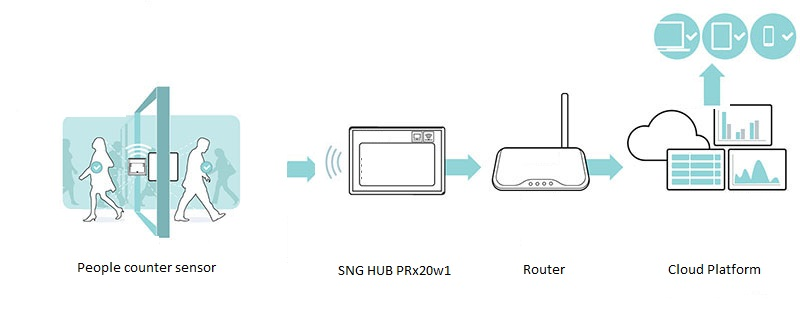
\includegraphics[width = 12cm,height = 5cm]{image/pc.jpg}
% \caption{People counter infrastructure used for our experimental dataset. Modified Figure of \protect\cite{SensM}}
% \label{people}
% \end{figure}


% \begin{table}[!h]{}
% \small
% \centering
% \caption{List of people counter sensors of International Road Dynamics company}%\cite{people}.}
% \begin{tabular}{llll}
% \toprule
% \textbf{Features} & \textbf{Transmitter} & \textbf{Receiver}  & \textbf{Applications}     \\
% \midrule
% Display/Wireless/Bidirectional     &  PTx20-1 & PRx20WD1 & Entrance and daily counts\\ 
% Wireless/Bidirectional             &  PTx20-1 & PRx20W1  & Entrance and daily counts\\ 
% Display/Bidirectional              &  PTx20-1 & PRx20D1  & Entrance and daily counts\\ 
% USB/Bidirectional                  &  PTx20-1 & PRx20U2  & Entrance and daily counts\\ 
% Display/USB/Bidirectional          &  PTx20-1 & PRx20UD2 & Entrance and daily counts\\ 
% \bottomrule
% \label{sensor}
% \end{tabular}
% \end{table}




% \subsection{Indoor Localization Using WiFi}

% Automatic user localization calculates the position of the user by knowing latitude, longitude, and altitude. This can be calculated by having an electronic device such as a mobile phone. Indoor localization is still a challenging topic, and it is because of the loss of GPS signals in indoor environments.

% Wireless-based indoor localization is another way for measurements. Wireless waves can go through obstacles like walls or doors and provide ubiquitous coverage of a building. WLAN indoor localization uses received signals value (RSSI) to indicate the distance to points and get the current point's location.
% This architecture needs two things, the beacon station that emits the wireless signals and electronic devices such as cellphones. 
% Fingerprint means the characteristic or feature of signals which RSS can be one of them. The assumption underneath this fingerprint-based indoor localization is that for each position in the area, the signals' features are different. By relying on the variation of signals in a distinct position, the current location can be obtained.



% ############################
% Two datasets that were obtained from short duration experiments lasting from a few days to a few months are analyzed in this thesis. The two experiments are the e-counter Indoor occupancy behavioural tests and the WiFi fingerprint Indoor Localization database. 
% Two case studies have been selected to evaluate the performance of the novel DSAP algorithm in a real-world scenario. Both the datasets analyzed in this work were part of short duration experiments lasting from a few days to a few months. 

% One method thought to increase incidental physical activity at work is the use of stair-promoting interventions. Stairs are readily available and stair climbing is considered vigorous physical activity. Motivational signs have been extensively and effectively trialled to increase stair use, but are they suitable for contemporary populations


%\subsection{E-counter Indoor Localization}

\section{Behavioural Intervention Experiment}

%Climbing stairs is an easy activity with proven health benefits which can be incorporated constructively in the lives of most people. 

Our first case study consists of an experiment performed in the Tonsley building at the campus of Flinders University, Australia in 2019. This study was conducted to observe the potential impact of motivational and educational interventions on the physical activity of people with sedentary lifestyles. 

% As part of the experiment, the number of people using stairs in the Tonsley building was monitored to study the stairs usage patterns. Nearly continuous measurements using e-counters were made over three months to infer any potential improvement in the stair usage after the introduction of motivational interventions. This included a month of undisturbed baseline measurements, a month of motivational intervention to increase stair use, and finally a month to observe the long term effect if any due to the intervention period. 





%The e-counter dataset used in this research was obtained from a behavioral intervention experiment to increase stair use that was The details of this experiment conducted in 2019 is described below.


%\subsubsection{Experiment}
 

%\begin{itemize}

% \item\textbf{Data Collection: }
%This experiment was conducted in the Tonsley Building over three months, that included a month of undisturbed baseline measurements, a month of motivational intervention to increase stair use, and finally a month to observe the long term effect if any due to the intervention period. 

Tonsley Building is a six-story building populated by students and staff with entrances facing North and South directions. The building floor layouts are illustrated in Figure \ref{laay}. The north-side entrance faces a small barricaded entrance as seen in panel \ref{laay:tpleft1}, but the main entrance is on the south side adjacent to the covered Tonsley garden. The building is fitted with lifts that reach all the levels, but also have stairs on the north and south sides that connect all the levels. Additionally, the building has an open space called the void and has central stairs that connect all the levels. Thus each level stairs are labeled as level $L_{x+1}-L_x$ North/South/Central, where $L_x = 1,2,.5$. 


\begin{figure*}[ht]
\centering
\subfloat[Google View of the building]{\label{laay:tpleft1}{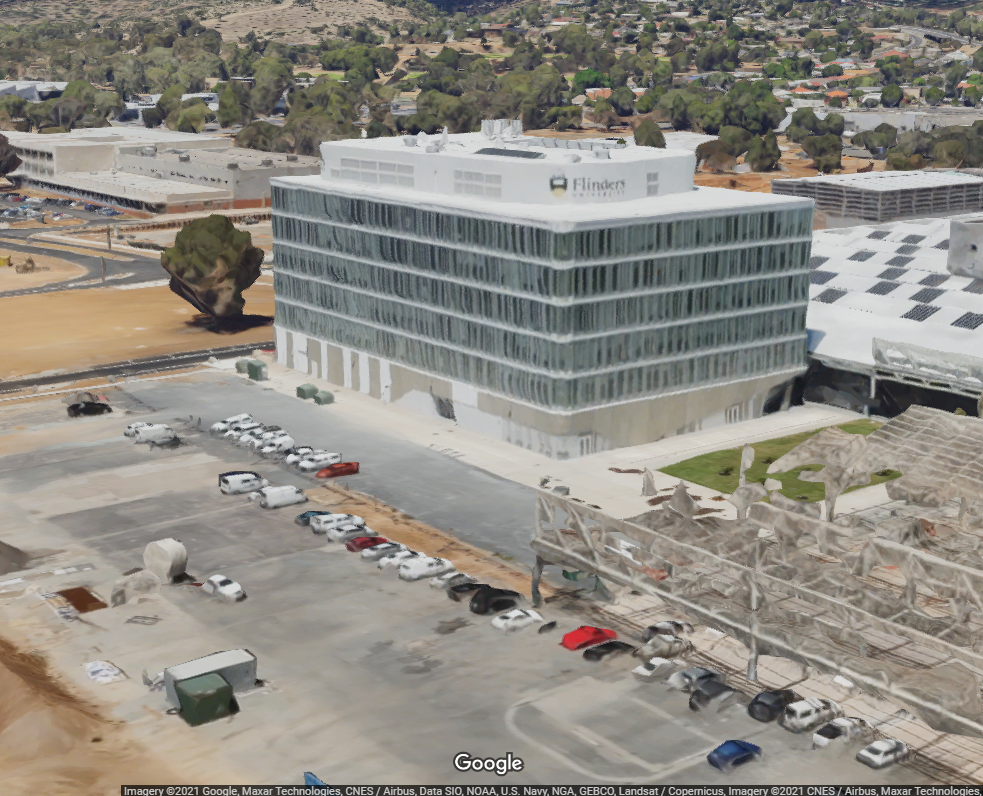
\includegraphics[width=5 cm, height = 4.2 cm]{image/Chapters/Chapter5/flinder.PNG}}}\hfill
\subfloat[Level 1]{\label{fig:md}{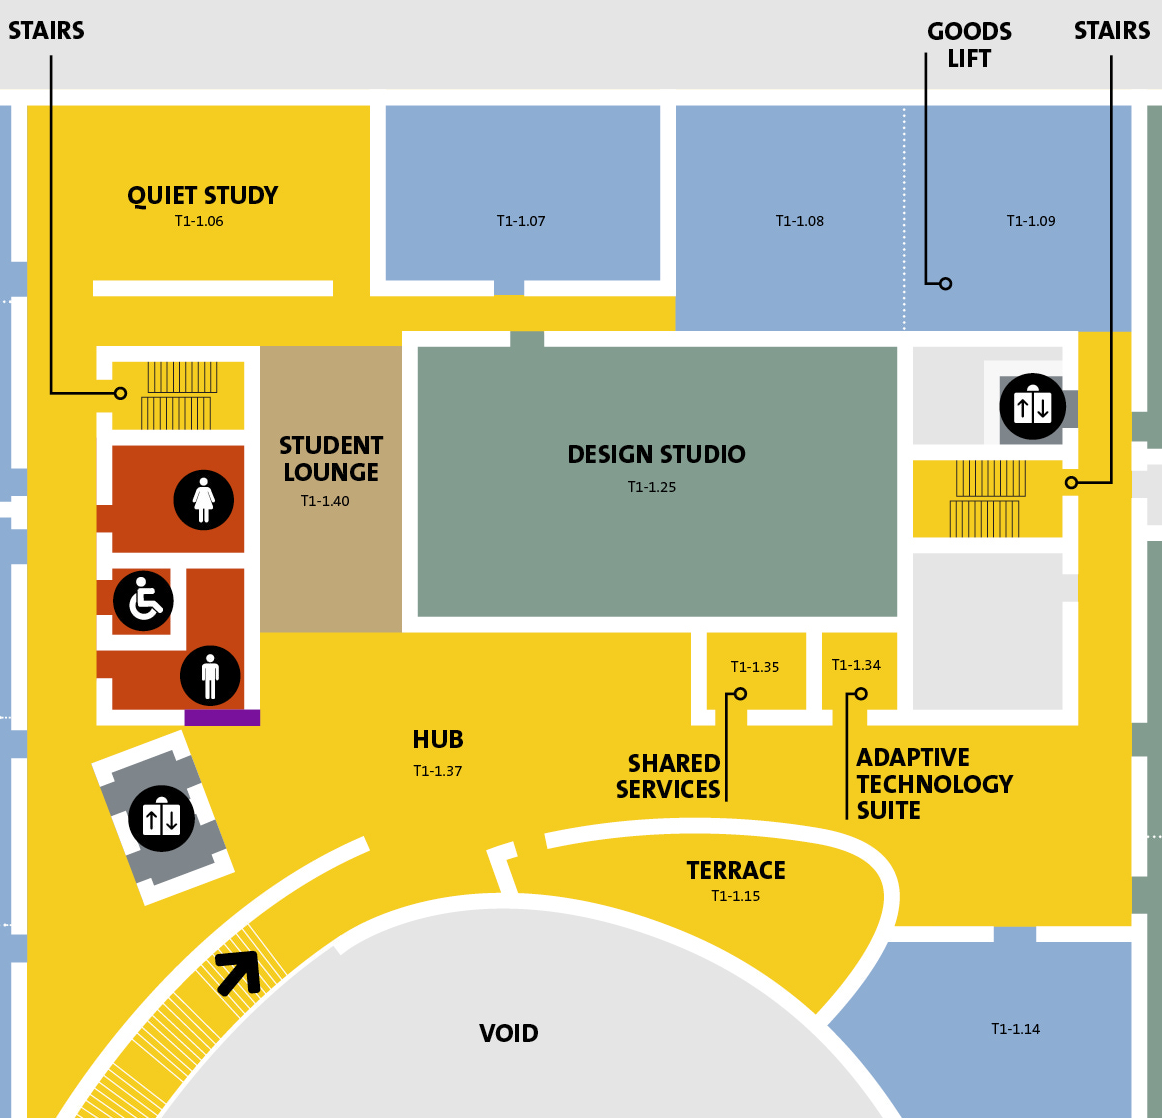
\includegraphics[width=0.3\textwidth]{image/T1.png}}}\hfill
\subfloat[Level 2]{\label{fig:mdright}{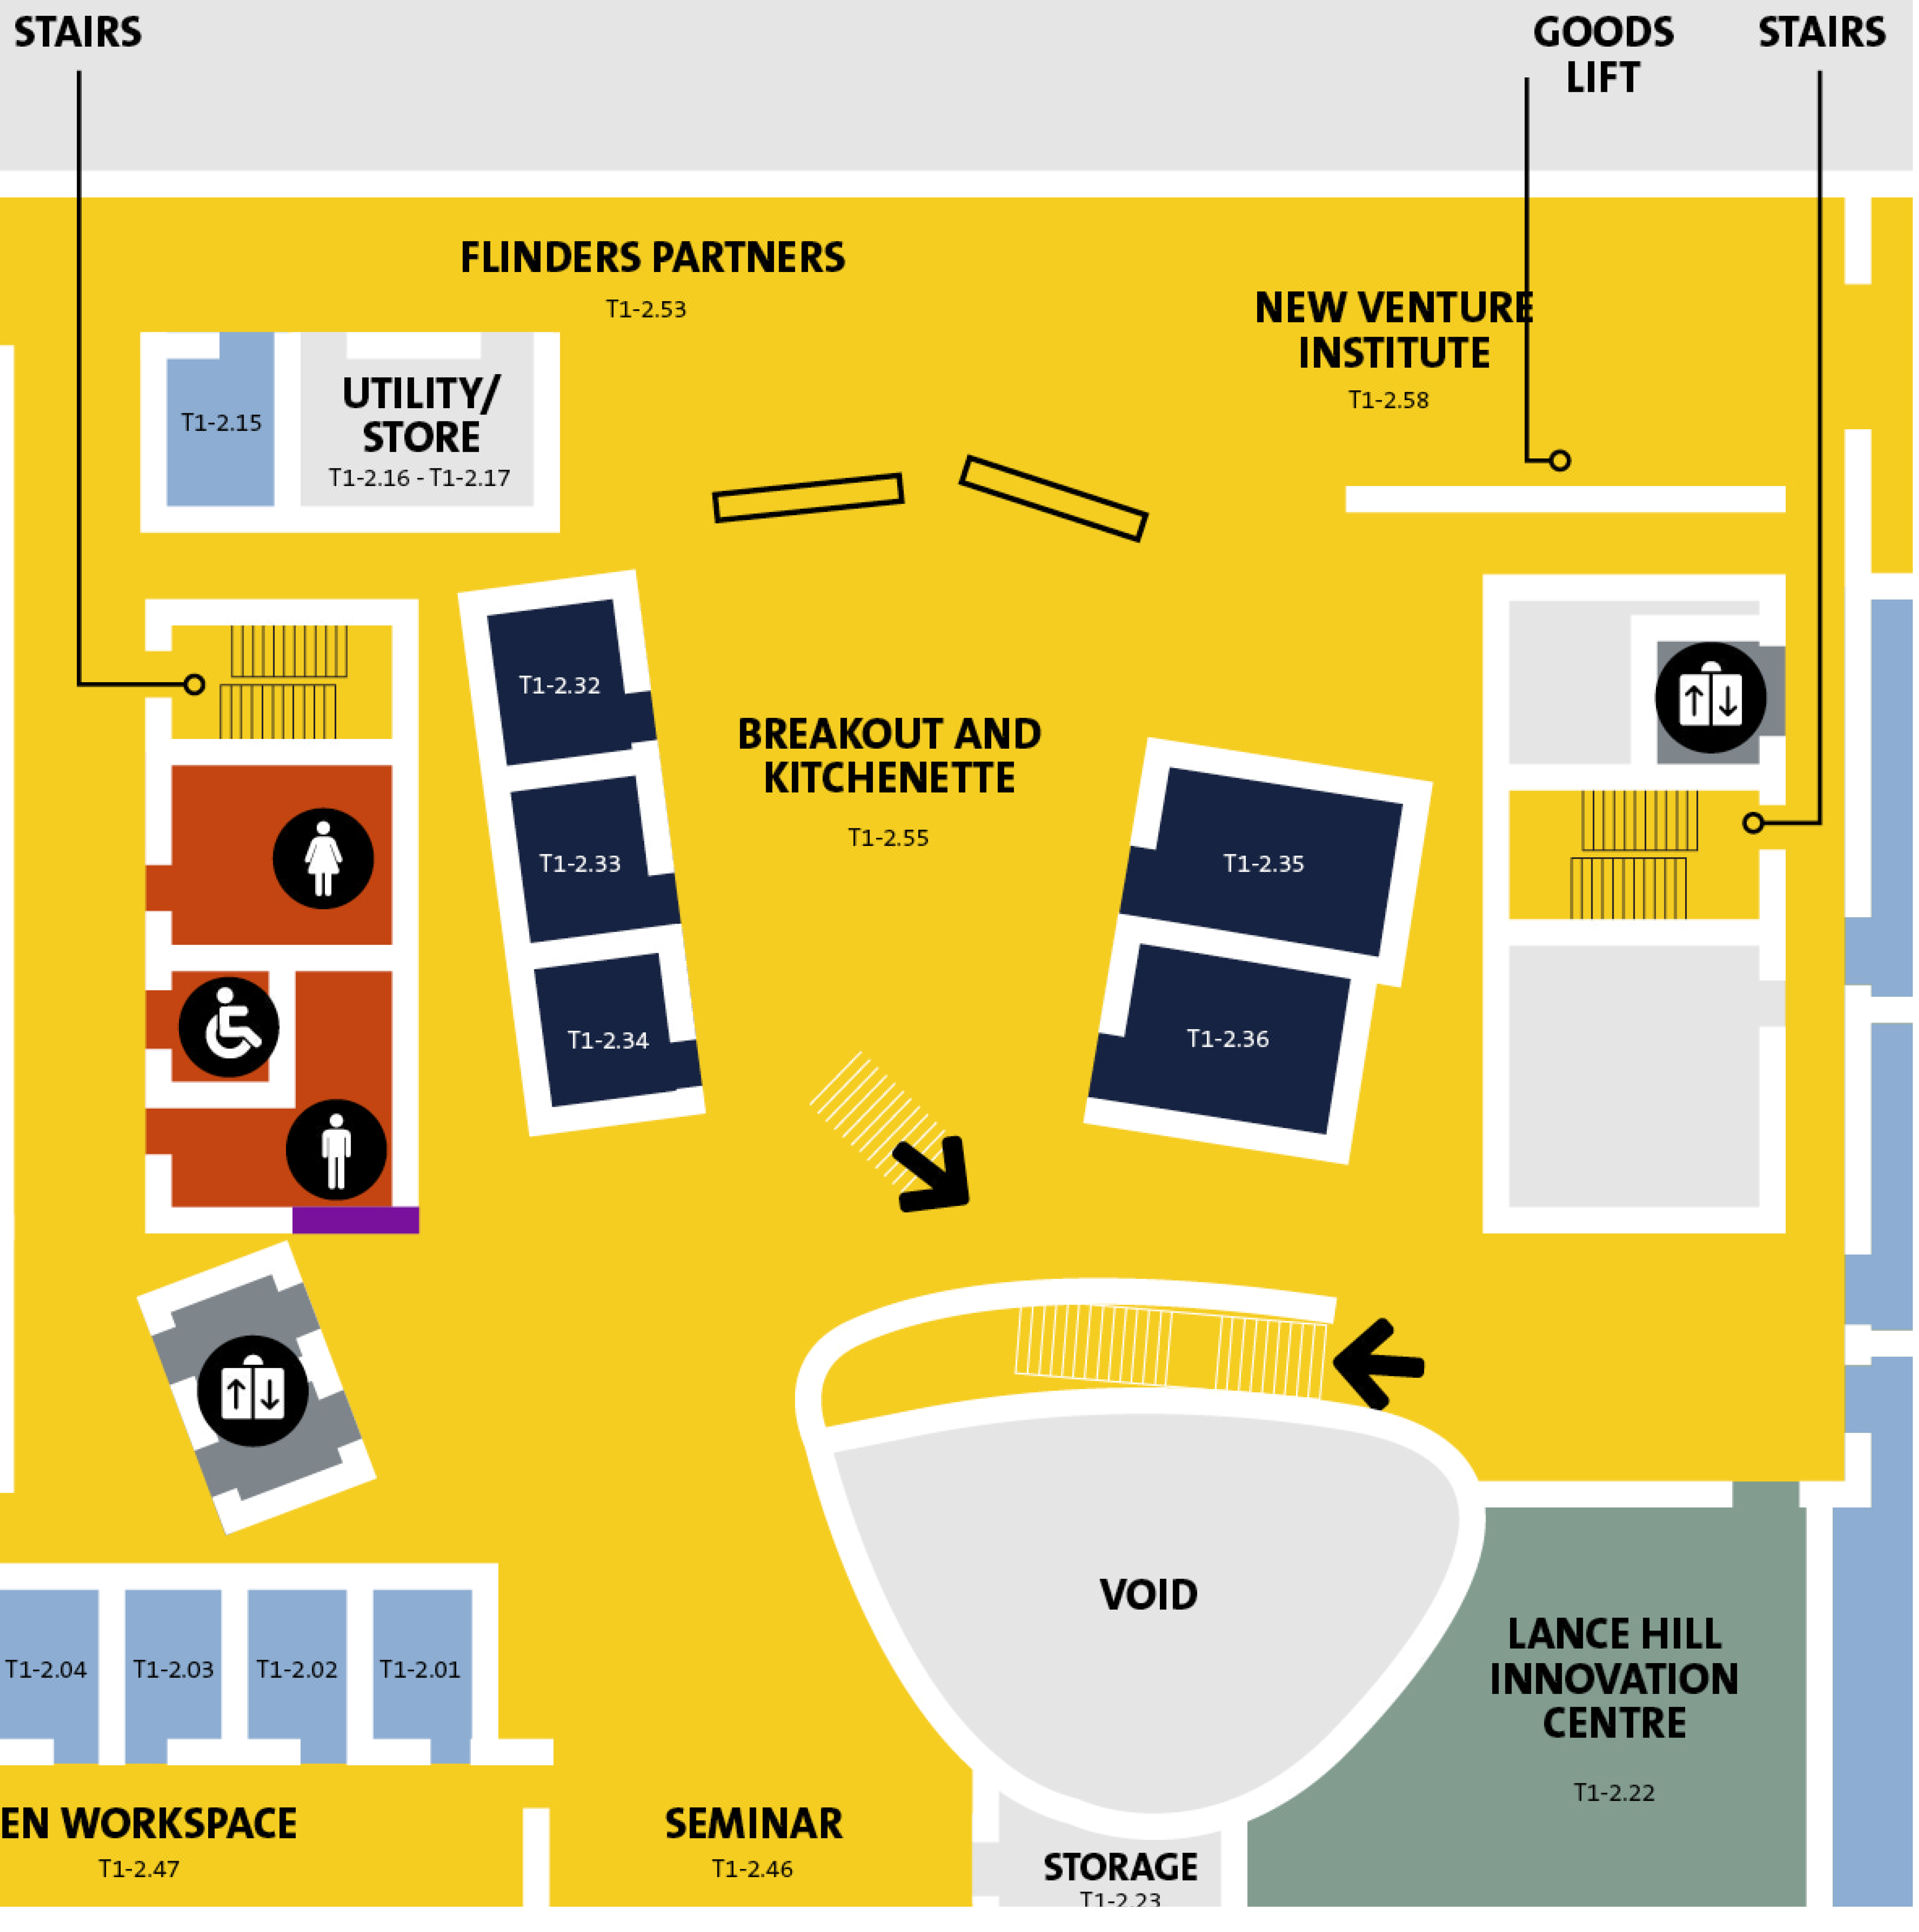
\includegraphics[width=0.3\textwidth]{image/T2.png}}}\hfill
\subfloat[Level 3]{\label{fig:btleft}{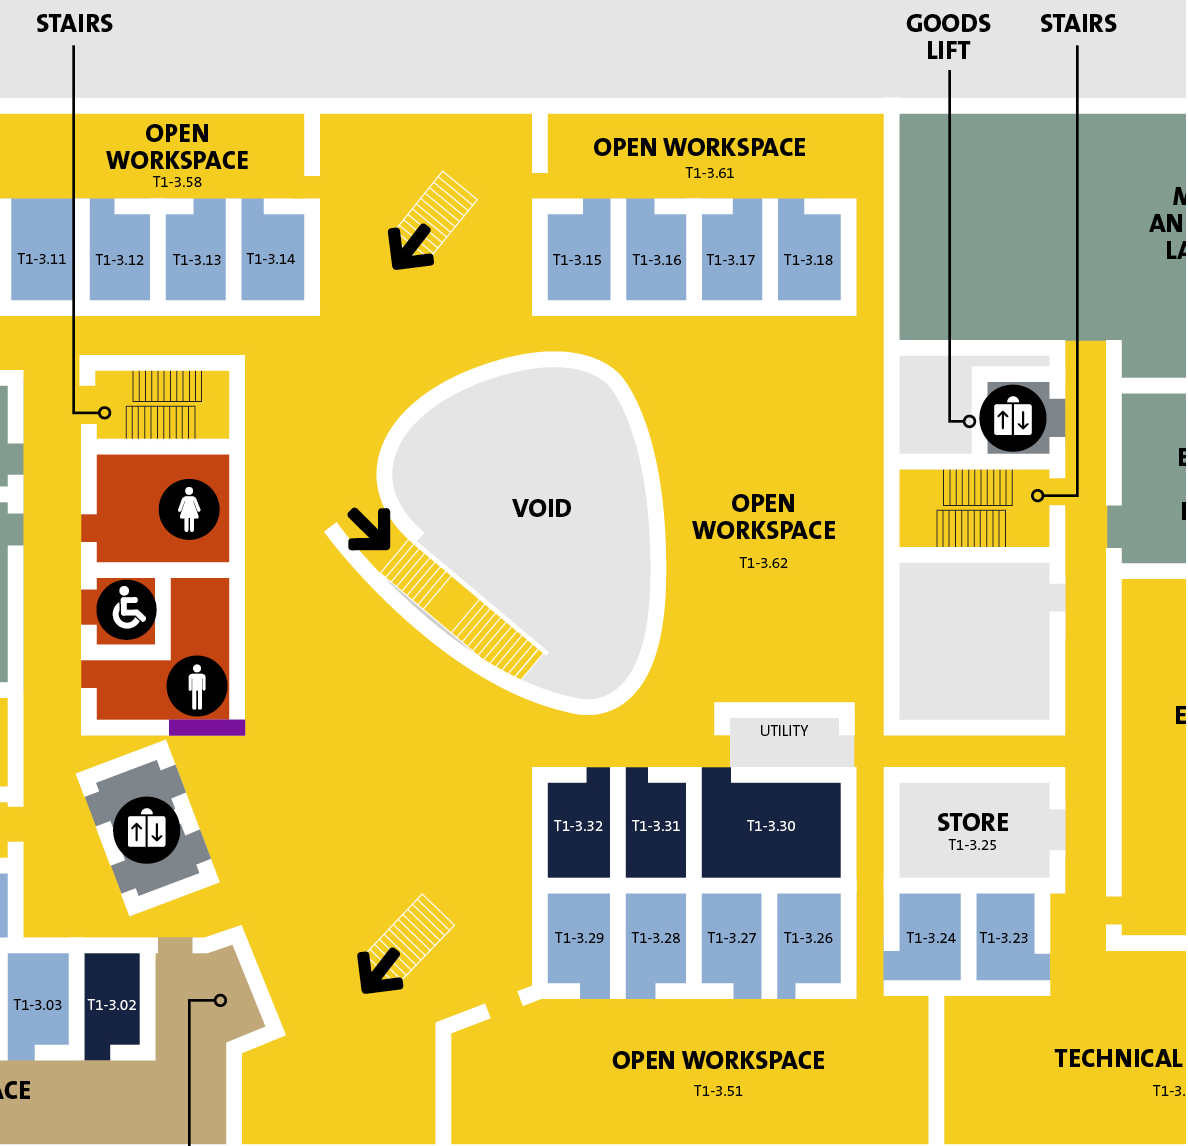
\includegraphics[width=0.3\textwidth]{image/T3.png}}}\hfill
\subfloat[Level 4]{\label{fig:md1}{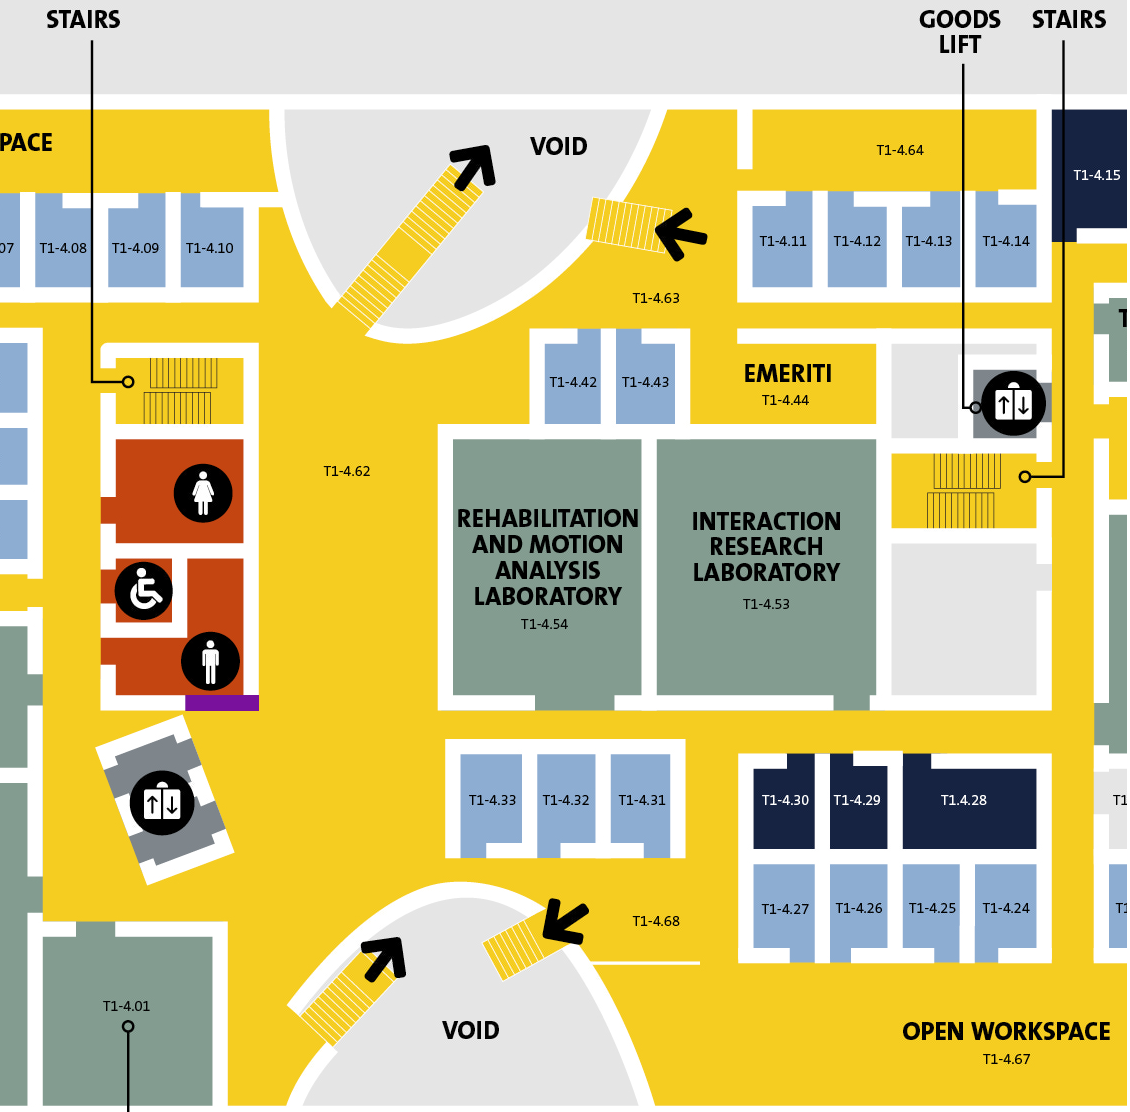
\includegraphics[width=0.3\textwidth]{image/T4.png}}}\hfill
\subfloat[Level 5]{\label{fig:mdright1}{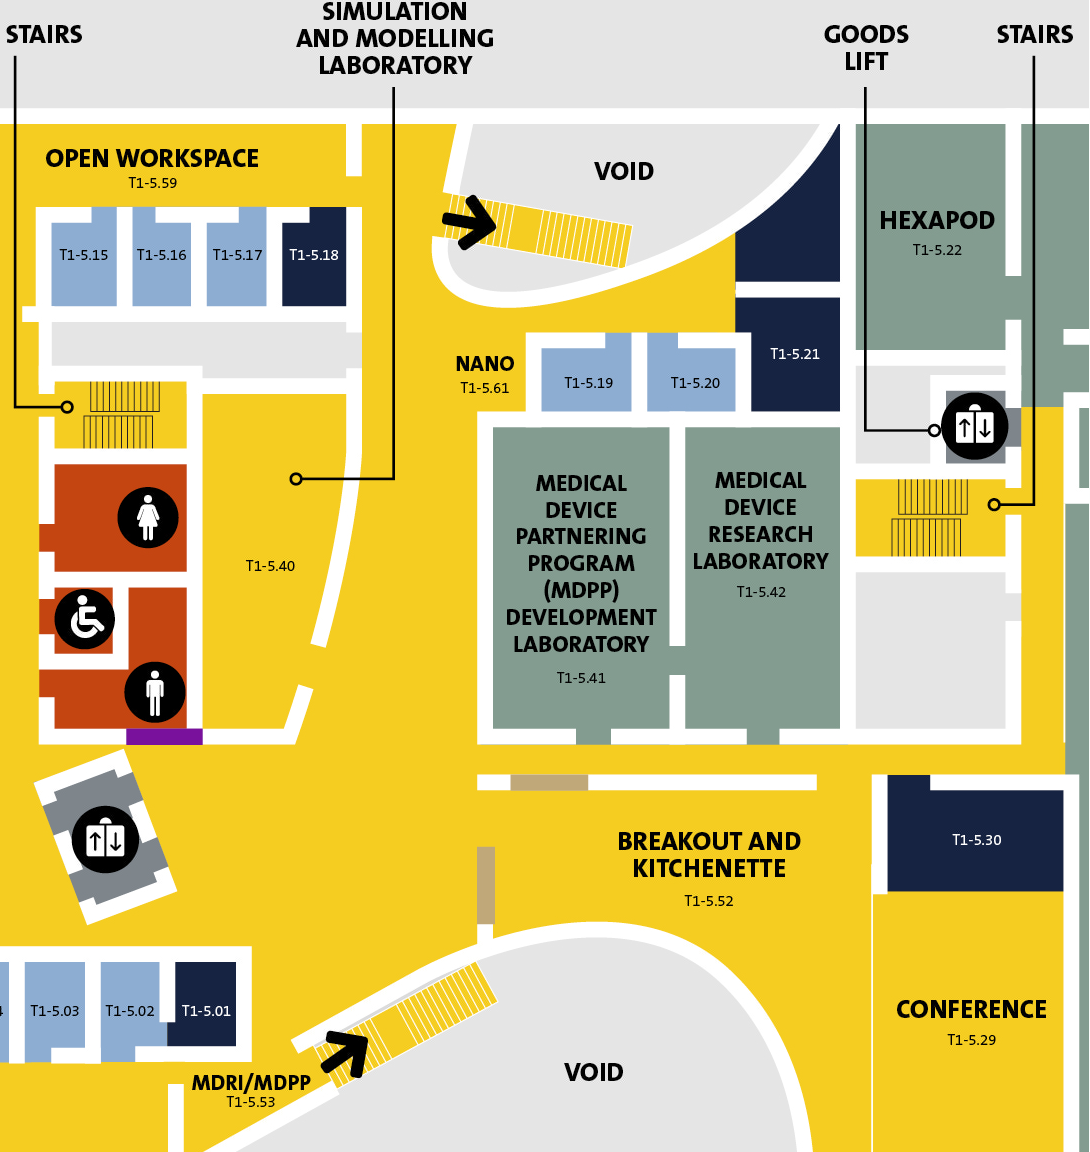
\includegraphics[width=0.3\textwidth]{image/T5.png}}}
\caption{Tonsley Building Layout. (a) Tonsley building view from the north-side parking lot, (b)-(f) Layout of levels 1-5.}
\label{laay}
\end{figure*}

E-counter sensors were deployed at all stairs. They are made by the International Road Dynamics company and consist of a pair of transmitter and receiver(transmitter: PTx20-1 and receiver: PRx20W1). The transmitter sends an infrared message to the receiver, when the infrared light is interrupted by someone passing through it, a count is registered. If no one passes, then these sensors log a count value of zero every 10 minutes. Each stair has two sensors, UP/DOWN that determine a person's direction of travel up and down the stairs. Signals from the sensors are sent to wireless hubs in real-time and then from the hubs to the server. The specification of all the sensors from this company are shown in Table \ref{sensor}. The maximum count value for each direction is about 1,000,000.

\begin{table}[!ht]
 \small
\centering
\caption{E-counter sensors of International Road Dynamics company}%\cite{people}.}
\begin{tabular}{llll}
 \toprule
\textbf{Features} & \textbf{Transmitter} & \textbf{Receiver}  & \textbf{Applications}     \\
\midrule
 Display/Wireless/Bidirectional     &  PTx20-1 & PRx20WD1 & Entrance and daily counts\\ 
Wireless/Bidirectional             &  PTx20-1 & PRx20W1  & Entrance and daily counts\\ 
 Display/Bidirectional              &  PTx20-1 & PRx20D1  & Entrance and daily counts\\ 
 USB/Bidirectional                  &  PTx20-1 & PRx20U2  & Entrance and daily counts\\ 
 Display/USB/Bidirectional          &  PTx20-1 & PRx20UD2 & Entrance and daily counts\\ 
 \bottomrule
 \label{sensor}
 \end{tabular}
 \end{table}



Each level has two types of location: level entrance and stairs. These entrances have two types of sensors: OUT/IN and two types of sensors for stairs as UP/DOWN. These are coded for all levels except level0-1, which is both a stair and an entrance, so it has the label UP/IN and DOWN/OUT, instead of either UP or DOWN (stairs) or IN or OUT (entrances).

%Data collection is the process of gathering and measuring information. The data collection method consists of two categories, quantitative and qualitative.Experimental research is a quantitative method. Interviews are qualitative methods.Surveys, observations, archival research and secondary data collection can be quantitative or qualitative methods.Hence, collecting streaming data needs time and facilities, we used two ready to use dataset and apply a stream simulation phase to use as data stream for our model.

%\subsection{E-counters Geographical Location}
%\subsubsection{People Counting Localization Indoor Dataset}

The data was collected from February 21, 2019, until July 16, 2019, but only three months of this data set was monitored for the experiment. The experiment was conducted for a period of three months from March 18 to June 23, 2019, as shown in Table \ref{tons}. During the first month period starting on March 18, 2019, data was collected to establish a baseline for staircase usage by making measurements as unobtrusively as possible. The mid-semester break from April 15-28 was excluded from the study. 

Motivational and educational interventions were made during the next month period starting from April 29, 2019 to increase stair usage. The interventions included digital screens that displayed health information and provided live feedback throughout the building, especially near the lifts. An additional month period starting on May 27, 2019 was observed in order to assess any long term changes in the stair use pattern after the end of the intervention period. To keep the stair usage experiment duration separate from the rest of the data, it is saved in a different .CSV file to be used for pre-processing. 
%which provides us with a valuable 3-month dataset to model stair usage in a campus environment.


\begin{table}[ht]
\setlength{\arrayrulewidth}{0.5mm}
\setlength{\tabcolsep}{18pt}
    \centering
    \caption{Experiment timeline at Tensely Building for three months of intervention. The green color shows the before intervention month, the blue color indicates the intervention month, and the yellow color represents the month after the intervention period. The red and pink colors represented anomalous periods and are out of scope for this experiment.}
    \label{tons}
    \begin{tabular}{c c c}
    \hline
     \textbf{Semester Weeks} & \textbf{Timeline} & \textbf{Date} \\
     \hline\midrule
    \rowcolor{green}
     week 12 &  Baseline(Before intervention)  &  3/18/2019 \\
     \hline
    \rowcolor{green}
     week 13 & Baseline  & 3/25/2019 \\
     \hline
    \rowcolor{green}
     week 14 & Baseline   & 4/1/2019 \\
     \hline
    \rowcolor{green}
    week 15 &   Baseline & 4/8/2019 \\
     \hline
     \rowcolor{pink}
        & Mid Semester Break  & 4/15/2019 \\
      \hline
     \rowcolor{pink}
      &  Mid Semester Break  & 4/22/2019 \\
     \hline
     \rowcolor{cyan}
     week 18 & Intervention  & 4/29/2019 \\
     \hline
     \rowcolor{cyan}
     week 19 & Intervention   & 5/6/2019 \\
     \hline
     \rowcolor{cyan}
    week 20 &   Intervention & 5/13/2019 \\
     \hline
     \rowcolor{cyan}
      week 21  & Intervention  &  5/20/2019 \\
      \hline
     \rowcolor{yellow}
     week 22 &  Follow-up(After Intervention)  & 5/27/2019 \\
     \hline
     \rowcolor{yellow}
     week 23 & Follow-up  & 6/3/2019 \\
     \hline
     \rowcolor{yellow}
     week 24 & Follow-up   & 6/10/2019 \\
     \hline
     \rowcolor{yellow}
    week 25 &   Follow-up & 6/17/2019 \\
     \hline
     \rowcolor{red}
        & Exams  & 6/24/2019 \\
      \hline
     \rowcolor{red}
        & Exams  & 7/1/2019 \\
      \hline
      \rowcolor{pink}
         & Semester Break  &  7/8/2019 \\
      \hline
      \rowcolor{pink}
         & Semester Break  & 7/15/2019 \\
      \hline
      \rowcolor{pink}
         & Semester Break  &  7/22/2019 \\
      \hline
      
    \end{tabular}
    
\end{table}



The sensors captured movement for all 24 hours and all days continuously. The raw e-counter data set consists of approximately 668,000 data points, each containing nine attributes as listed in Table \ref{attr} out of which almost half the data points were included in our research work. 


\begin{table}[!ht]
\centering
\caption{List of attributes for the e-counter data set}

    \begin{tabular}{p{2cm} p{3.5cm}  p{4.5cm} }
    \hline
    \textbf{Attribute} & \textbf{Measurement} & \textbf{Definition}\\ \hline
    \midrule
Date             &  mm/dd/yyyy      &   Date of measurement                                 \\\hline
Time             &  hh:mm:ss 24H    &   Time of measurement                                 \\\hline
Count            &  integer         &   Number of people counted by the sensor              \\ \hline
Sensor           &  Up, Down, In, Out, IN/Out-reserved & Direction of the sensor             \\ \hline
Position         &    string         &   Sensor location in the building                                                                                                      \\ \hline
Location Code    &     H2-L3             & Code for each location                                                                                                                                       \\ \hline
    \bottomrule
    \label{attr}
\end{tabular}
\end{table}





%The total number of people using the stairs over the entire experiment duration is shown in figure 2. It is apparent that people prefer taking the stairs to go down. An expected periodic lower occupancy is also observed on the weekends. The mid-semester break from April 15-28 was excluded from the study.


%\item\textbf{Data Pre-processing:}
During pre-processing, some issues were detected during the experiment period that affected the quality of our model. For instance, hubs were temporarily switched off or sensors fell off. Also, some special events took place during the experiment, such as public holidays, term breaks, and fire drills which affected the number of people using the stairs. For example, on May 1$^{st}$ at 11:15 a.m, the fire alarm went on, and everyone had to evacuate the building using the stairs. Also, between baseline duration and initiation of intervention, there was a two-week Easter break or semester break and that is why the intervention started after two weeks of the first stage. The data collected during the interrupted days mentioned above have not been included in the cluster analysis.

Furthermore, if no one passes through the beam of sensors, the sensors indicate zero during that specific interval. A huge number of zeros were logged during the experiment especially after working hours, weekends, and holidays, which could bias the clustering results. These zero values were removed from the data set. 

The e-counters save the position values as a string character combination of numbers and strings. Hence, it was also necessary to convert the string format of the position values into the integer format in order to allow us to use them as an input for the DSAP algorithm. 
%or fire alarm went to alarm for evacuation. This leads to having missing data points during data stream.%In addition, on May 7, printer level 5 broken and people had to use the stairs to get printer level 4.
Finally, the feature selection task was performed to provide a target data set ready to be used by the simulation and clustering. The Position and Count features were selected for computing the clusters. The hyperparameters for the AP in the DSAP algorithm are consistent and fixed for the entire experiment. The damping value is equal to 0.96, maximum iteration is 100, and preference is equal to the median of the similarity matrix.



% \begin{table}[!h]{}
% \centering
% \caption{Selected input variables for clustering the e-counter dataset.}

%     \begin{tabular}{p{3cm} l p{3cm} l  p{3cm} }
%     \hline
%     \textbf{Attribute} & \textbf{Description} & \textbf{Values} \\ \hline
%     \midrule
%      Position             &   The location of sensors installed in this building     
%      & Level2-1, Level3-2Central, Level4-3North, Level4-3South, Level5-4North, Level5-4South \\ \hline
%      Count               &  Number of people pass through the sensors    &   Integer:1,...n \\
%     \hline
%     \bottomrule
%     \label{variab}
% \end{tabular}
% \end{table}



%\item\textbf{Data Stream Simulation:}
%In order to mimic the data coming from an infinite stream, it was necessary to convert the limited duration into a data stream. The data stream simulation tools that are used are Scikit-Multiflow in Python and DSD in R. The reason why we have chosen these two simulations is that the DSAP algorithm has developed in Python, and the streaming K-means is implemented in the R programming language. 
%The target input dataset used for gathering the stream simulation is demonstrates in Table \ref{datain}. 

%To implement data stream for the DSAP algorithm with Scikit-Multiflow, we applied \textit{skmultiflow.data.FileStream} class for generating data stream out of our e-counter CSV file. The input of this class is a window with the size of l data point. Streaming K-means simulates data stream with Data Stream Data (DSD) object is used the package \textit{'stream'} by applying the \textit{DSD\_ReadCSV} function, which is a connector to the real-world data. The input of this function is the e-counter CSV file, and the output is a list of data points which the window updates every time frame by applying \textit{Update} function.

% \begin{table*}[ht]
% \centering
% \caption{the input data for the stream simulation.}
% \begin{tabular}{clclclc}
% \toprule
% \textbf{Date} & \textbf{Time} & \textbf{Position} &\textbf{Count}     \\
% \midrule
% 3/18/2019             & 8:12:31      &      4    &      1       \\
% 3/18/2019             & 8:32:31      &      4    &      2       \\
% 3/18/2019             & 8:52:31      &      4    &      1       \\
% ...                   &  ...         &      ...  &      ...     \\
% ...                   &  ...         &      ...  &      ...     \\
% 6/23/2019             & 19:13:01     &      6    &      1       \\
% 6/23/2019             & 19:23:01     &      3    &      1       \\
% \bottomrule
% \label{datain}
% \end{tabular}
% \end{table*}

%main itemize

%\end{itemize}


%%%%%%%%%%%%%%%%%%%%%%%%%%%%%
% I think we can remove this subsection. I can explain in next chapter
% \subsubsection{Data Stream Clustering}
% The measurements from the e-counters were analyzed to find patterns in time and space. Clusters of similar measurements with respect to position and count were generated using the DSAP and streaming K-means algorithms. To initiate the clustering algorithms, the size of the landmark time window needs to be defined. Different windows sizes ranging from 1 hour to 30 hours were test with the DSAP algorithm. A reasonable compromise between speed and accuracy of clusters was obtained for a window size of 5 hours, hence this was chosen as the size of the landmark window.% and because the number of people using the stairs are usually not significant or after working hours there is not much commuting, we consider each window with the length of 4 hour.
% There are several hyper parameters that need to be set in order to use the DSAP and streaming K-means algorithms correctly. This values are a function of the dataset under study. 
% \begin{itemize}
%     \item The damping factor for AP algorithm is constant for all AP function called and is equal to 0.9
%     \item The maximum iteration is the predefined value and it is 100.
%     \item The preference hyperparameter is the median value of the similarity matrix.
%     \item The expiration value equal to forget older windows is the last 5 landmark window (If it was applied). 
%     \item The landmark time frame is equal to every 5 hours.
% %    \item For the streaming k means algorithm the number of the macro clusters was obtained by the elbow method. This number is $k$ = 6 for the entire dataset.
% \end{itemize}












%  The same landmark window was used in the online clustering phase to generate micro-clusters. Once the data stream ended and all the micro clusters have been stored, the DSC function generation was again used for the computation of the macro clusters in the offline macro clustering Phase. 


%The data frame used for this dataset is every 4 hours. 

% \begin{itemize}
%     \item Preference parameter: the median value of the similarity matrix.
%     \item Damping factor: is equal to best result and reach convergence.
%     \item Maximum number of iteration and Convergence iteration: default values.
%     \item Threshold (comparing each new data point with the model): the minimum distance of data points to the centroids.

% \end{itemize}
   
% The online clustering initialises with 200 data points where gradually over time new data points are introduced and old data points are disposed. Micro-clusters were generated in each of these windows using the DSC function generation, and stored once the sliding window passed over the 200th data point relative to the starting data point.

% With a fixed number of cluster k = 4, for each landmark time window based on elbow method have been done separately, and once the data stream is ended and the micro clusters stored, the DSC function generation was again used for the computation of the macro clusters in the offline macro clustering Phase.

% In the end, to evaluate the performance of the clustering and compare two algorithm's clustering result for the e-counter dataset, different metrics are applied. Silhouette Coefficient, Calinski-Harabasz Index, and Davies-Bouldin Index, are calculated with two metrics obtain from clusters: cluster centroids and cluster labels. Processing time is calculated by subtract the end time from starting time with the  $time()$ method. Memory usage obtained from $psutil$ library in Python for processes and system utilization as same as $memory$ in R programming language. 

% We will go through these two stages below. 
    
%     \begin{itemize}
%         \item\textbf{DSC\_Window:} provides a clustering interface to the data stream operator $DSC\_Window$. It implements the sliding window model, which keeps a specified number of the most recent data points of the stream defines by the user. This number is the window length. 
        
%         \item\textbf{DSC\_Kmeans:} interface is the R version of K-means clustering implementation and a version of k-means where the data points (micro-clusters) are weighted by the micro cluster weights. The streaming k-means clustering algorithm requires continuously update the calculation of micro clusters.
        
%         For e-counter dataset, we used elbow method to find out the number of clusters which is equal to $k$ = 6. Also, same as the DSAP algorithm, the 10 minutes time frame was taken as a size of window. Once the data stream finished and the micro clusters collected all data points during this phase, the DSC function generation is used again to compute the macro clusters in the offline phase.
        
%     \end{itemize}
    

% \subsubsection{Clustering Performance Evaluation Phase}
% In order to compare the performance of the DSAP algorithm with streaming K-means clustering, the evaluation criteria discussed earlier in Section 4.4, were implemented using Python and R libraries. All the metrics implemented in Python are part of the $'Sklearn.metrics'$ library in Python and $'clusterCrit'$ in R including score functions and performance metrics. The input for Silhouette Coefficient, Calinski-Harabasz, and Davies-Bouldin Indexes are two parameter: centroids and label of clusters. The centroids are the output from streaming algorithms and the labels are predicted labels for each selected centroids. The output of each score is a floating number related to the clusters.

% The execution time of the clusters is another measurement to compare both DSAP and streaming K-means together. For the DSAP we used \textit{time()} function and for streaming K-means \textit{system.time} was used.

% Memory profiler in Python module for monitoring memory consumption of a process as well as line-by-line analysis of memory consumption for Python programs is used to estimate the memory consumption. It is a pure Python module that depends on the 'psutil' module. It first decorates the function you would like to profile with @profile and then runs the script with a special script (in this case with specific arguments to the Python interpreter).


    % \item \textbf{Silhouette Coefficient:} 
    %     \begin{itemize}
    %  \item  DSAP:
    %       \item Streaming K-means:
    %  \end{itemize}
    
    %To compute this factor for both Python and R programming language, we used Silhouette function the code below:
    % \begin{equation}
    %     sklearn.metrics.silhouette\_score(X, labels, *, metric='euclidean', sample\_size=None, random\_state=None, **kwds)
    %  \end{equation} 


% \begin{figure}
% \centering
% 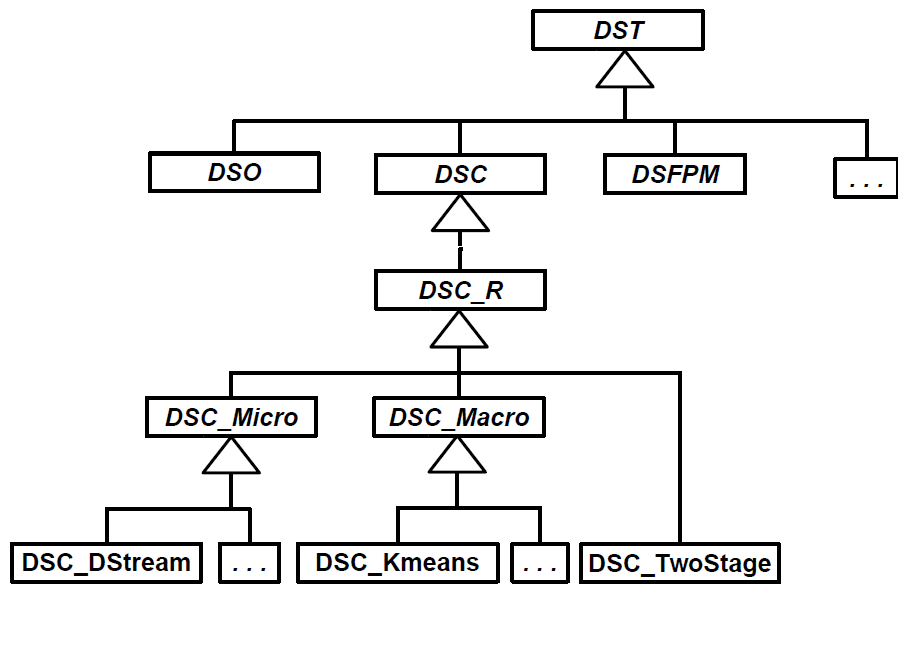
\includegraphics[width = 15cm,height = 9cm]{image/dst.png}
% \caption{Overview of data stream task (DST) \cite{hahsler2017introduction}. Overview of the data stream Data (DSD) class structure and data stream clustering (DSC) class structure with sub-classes.}
% \label{DSD}
% \end{figure}

%%%%%%%%%%%%%%%%%%%%%%%%%%%%%%%%%%%%%%%%%%%%%%%%%%%%%%%%%%%%%%%%%%%%%%%%%%%%%%%%%%%%%%%%%%%%%%%%

\section{Occupant Behaviour Experiment }\label{wifidat}

%The ubiquitous presence of wireless networks has brought opportunities for detecting non-intrusive human activity in an indoor environment. A significant advantage of the WAN fingerprint-based methods is that no additional hardware is needed as they use the existing WLAN infrastructure for position estimation. Therefore, the location of the user can be achieved without any expensive additional infrastructure. Accurate estimation of indoor location has applications in many areas including marketing, tracking products, assistance service in hospitals, etc. The WLAN Fingerprint-based Indoor Localization dataset, called UJIIndoorLoc dataset \cite{torres2014ujiindoorloc}, was one of the first publicly accessible and multi-storey database  to compare different indoor localization methodologies.  This experiment was conducted at the Universitat Jaume I (UJI), Spain, in 2013.

% \begin{figure}
%   \centering
% \sidesubfloat[]{\label{main:a}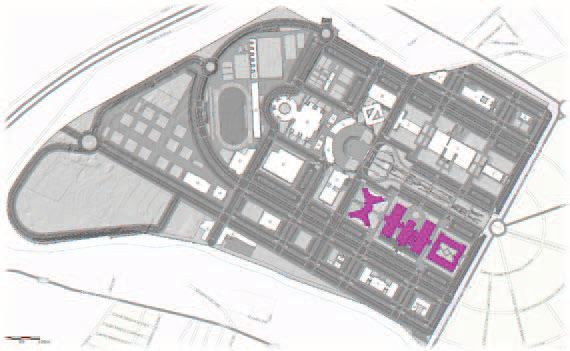
\includegraphics[width=0.4\linewidth]{image/uj1.png}}
%  \sidesubfloat[]{\label{main:b}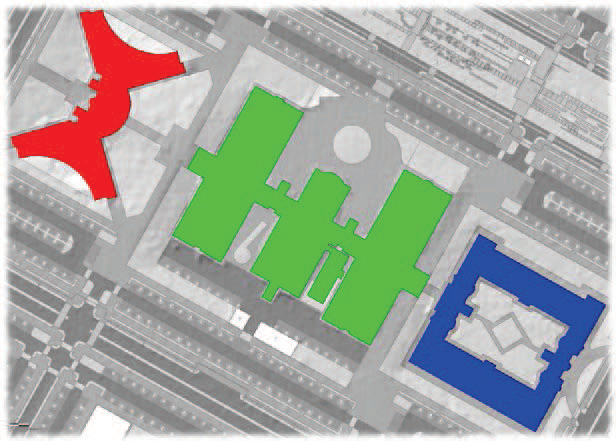
\includegraphics[width=0.4\linewidth]{image/uj2.png}}
% \bigskip
%     \caption{(a) Map of the UJI Riu Sec Campus and the buildings used for this experiment with purple color. (b) A zoom of these three buildings, T1 building show with the red color, TD building shows with the green color, and TC building shows with the blue color.}%\cite{torres2014ujiindoorloc}
%  \label{uji}
% \end{figure}


% \begin{figure*}[]%htb
% \begin{minipage}{.5\textwidth}
%   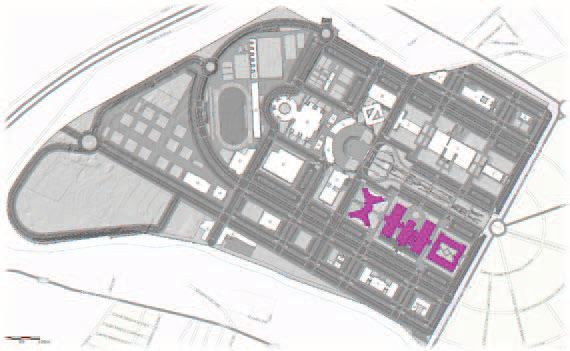
\includegraphics[width=1\textwidth]{image/uj1.png}
% \end{minipage}%
% \hfill
% \begin{minipage}{.5\textwidth}
%   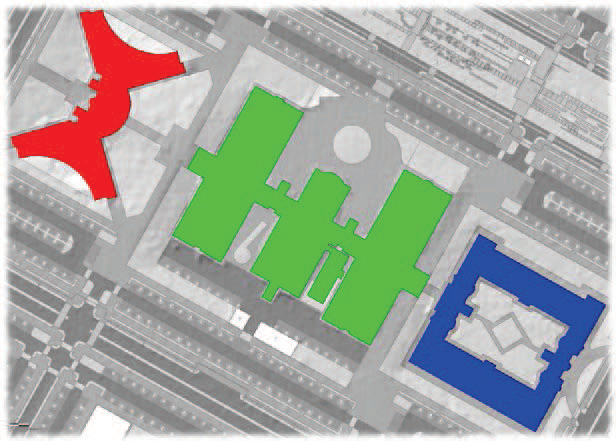
\includegraphics[width=.9\textwidth]{image/uj2.png}
% \end{minipage}
% \hfill
% \caption{(a) Map of the UJI Riu Sec Campus and the buildings used for this experiment with purple color. (b) A zoom of these three buildings, T1 building show with the red color, TD building shows with the green color, and TC building shows with the blue color.}
% \label{uji}
% \end{figure*}




%\subsubsection{Experiment}
% This experiment covers three buildings of Universitat Jaume I. It was created in 2013 by means of more than 20 different users and 25 Android devices.
% Samples were taken from random position

This case study was carried out to find occupant  behavior patterns  in  indoor  spaces  to provide  relevant  information  for  future planning  building  automation, evaluating energy efficiency scenarios, and simulating   emergency   protocols. The experiment was conducted over four months at the Universitat Jaume I campus, in Valencia, Spain. During this time, users carried mobile devices that used \textit{CaptureLoc} to record eight types of attributes including user position and WiFi signal strength across a total of thirteen levels spanning three buildings of the campus. To protect the identity of the participants during the course of the experiment, the unique MAC identifiers of the phones were hashed (anonymized) on reception.
%\begin{itemize}

%\item\textbf{Data Collection:}

% This experiment was conducted over four months at the UJI university campus and was divided in two sections: Training set and Validation set. 

The UJIIndoorLoc data set generated includes three buildings with four or more floors (one building has five floors) and almost 110.000 m$^{2}$of space. The total number of locations captured was 933. The shape and structure of the three buildings TI, TD, and TC, are quite different, as shown in Figure \ref{dspp2}. The raw data set consists of 19,938 data points containing 529 attributes as illustrated in Table \ref{featuj}. %These attributes include the Received signal strength indicator (RSSI) for 520 wireless access points (WAPs). The RSSI is an unitless number that provides an estimates of the  received signal strength.


\begin{figure*}[!ht]
\centering
\subfloat[Overview of the three buildings]{\label{fig:build}{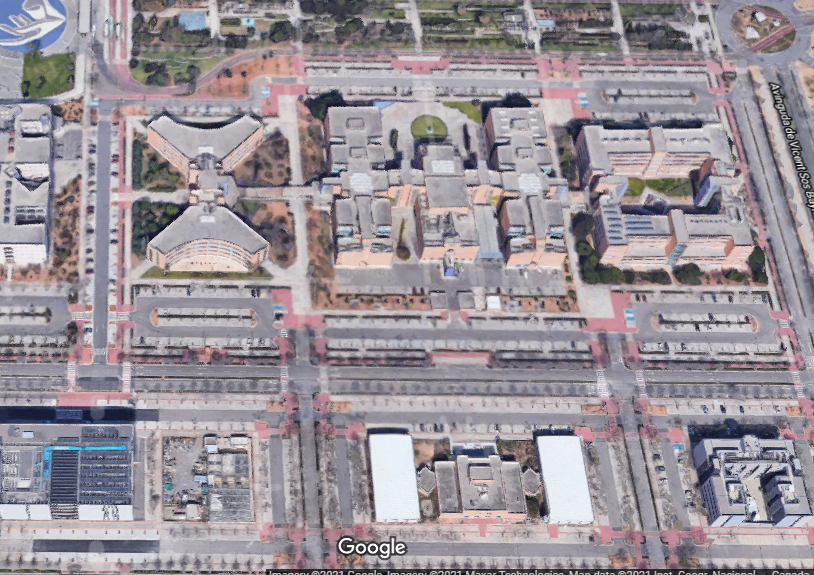
\includegraphics[width=7 cm, height = 6 cm]{image/Chapters/Chapter5/uji.PNG}}}\hfill
\subfloat[Building Number 0 (TI)]{\label{fig:bl2}{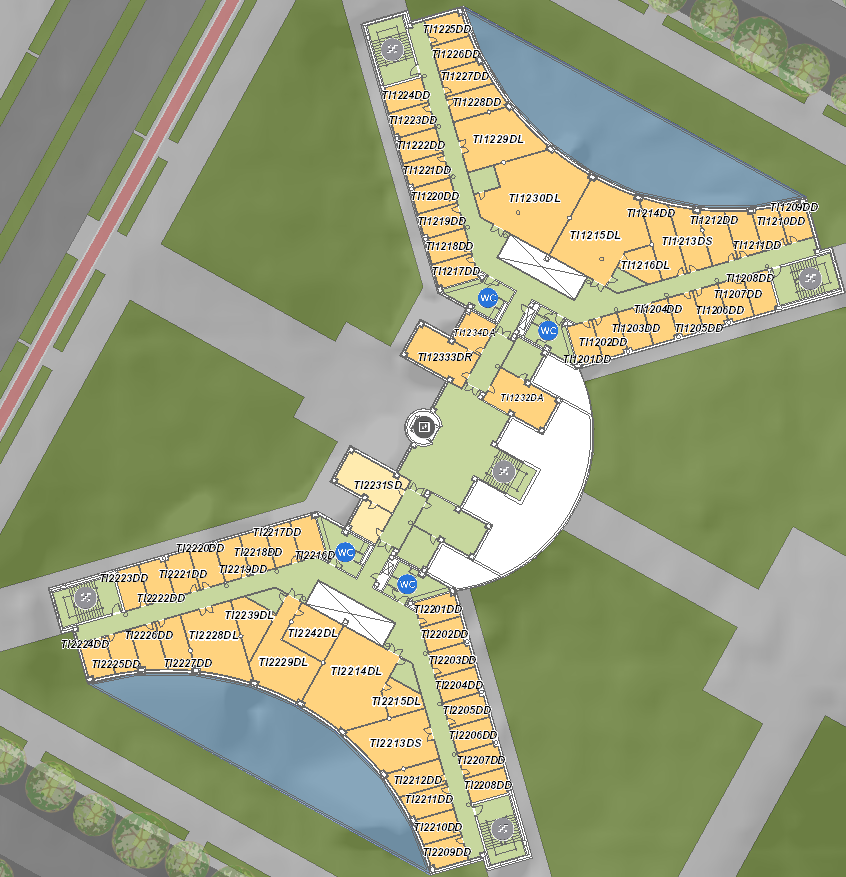
\includegraphics[width=0.4\textwidth]{image/plan2.png}}}\hfill
\subfloat[Building Number 1 (TD)]{\label{fig:bl3}{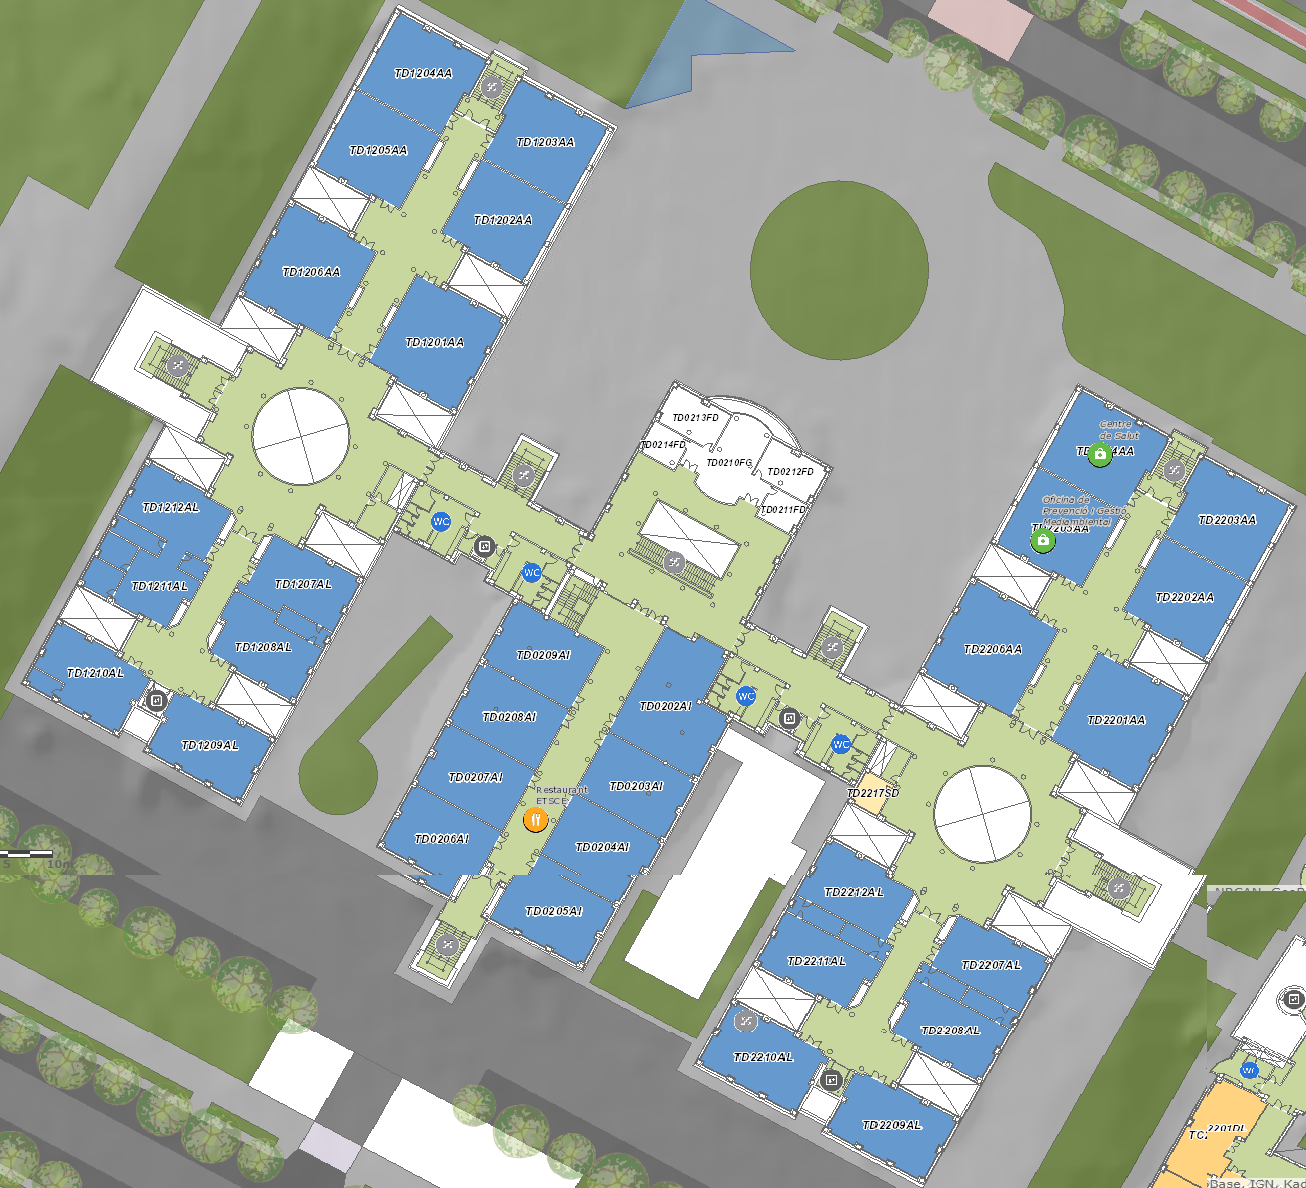
\includegraphics[width=0.4\textwidth]{image/plan3.png}}}\hfill
\subfloat[Building Number 2 (TC)]{\label{fig:bl4}{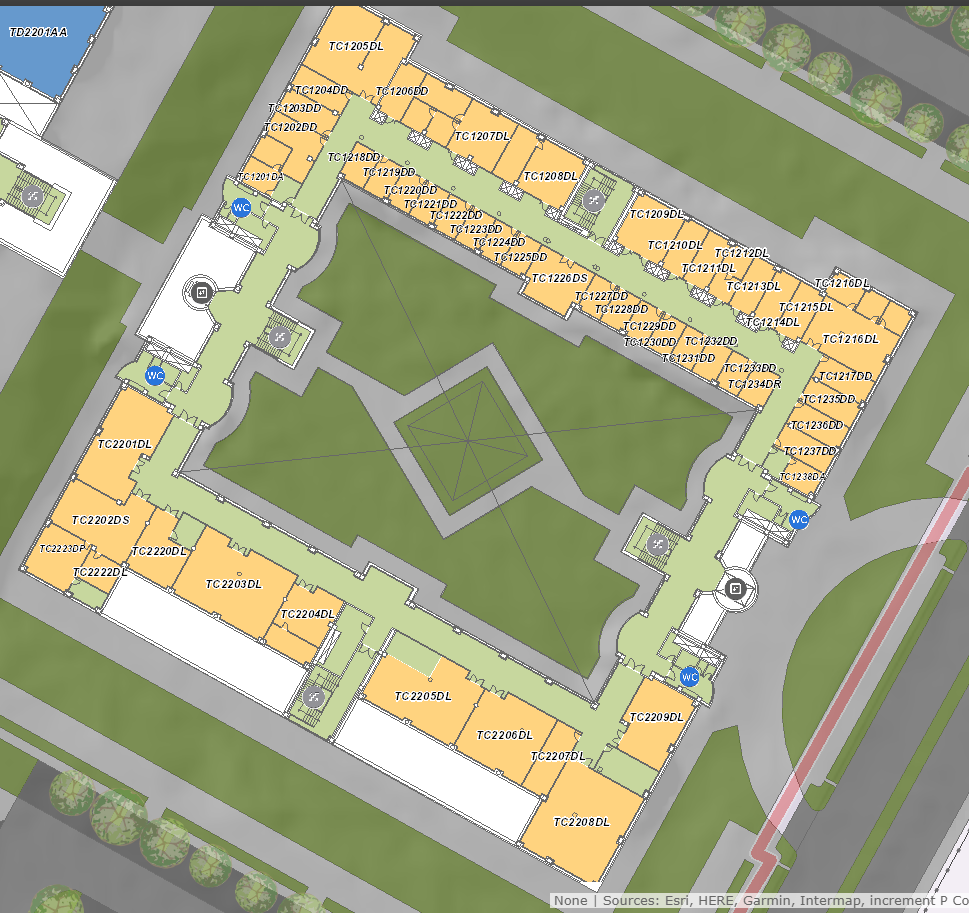
\includegraphics[width=0.4\textwidth]{image/plan1.png}}}\hfill
\caption{(a) Map of the UJI Riu Sec Campus and the buildings used for WiFi fingerprint experiment. (b,c,d) The layout of the three buildings with spaceid numbers for a floor.}% is shown with purple color. A zoom of T1, TD, and TC building shows. Inside the plans we have information regarding spaceID.}
\label{dspp2}
\end{figure*}

%***** remove 
\begin{table}[!ht]
\centering
\caption{ List of attributes of the UJIIndoorLoc data set.}
\small
    \begin{tabular}{ p{4cm} p{4.5cm} p{4.5cm} }
    \hline
    \textbf{Attributes} & \textbf{Measurement} & \textbf{Definition} \\ \hline
    \midrule
    RSSI Level             &    -100dBM: weak signal, 0dBM: good, 100dBM: not detected    & RSSI levels where the WAP identifiers are linked to the vector positions           
    \\\hline
    Longitude              &    UTM from WGS84     &  Y coordinates           \\\hline
    Latitude               &    UTM from WGS84     &  X coordinates          \\\hline
    Floor                  &    0,1,2,3,4     &  Floors of each building           
    \\\hline
    Building ID            &    0,1,2     &  Each of the three buildings TI,TD, and TC          
    \\\hline
    Space ID               &    integer   & Identification of an indoor space (e.g. room or corridor)            
    \\\hline
    Relative Position      &    1= inside 2=outside       & Outside means in front of the door of the space \\\hline
    User ID                &    0,1,2,...,18    &  Unique code for users who participated in the experiment           \\\hline
    Phone ID               &    0,1,2,...,24      &    Android device code used for this experiment        \\\hline
    Timestamp              &    Unix time format      &  Time of capture           
    \\
    \bottomrule
\label{featuj}
\end{tabular}
\end{table}


% \\
% \textcolor{blue}{001-520: } RSSI levels\\
% \textcolor{blue}{521-524: } Real world coordinates of the sample points\\
% \textcolor{blue}{524: }\hspace{.75cm} BuildingID\\
% \textcolor{blue}{525: }\hspace{.75cm} SpaceID\\
% \textcolor{blue}{526: }\hspace{.75cm} Relative position with respect to SpaceID\\
% \textcolor{blue}{527: }\hspace{.75cm} UserID\\
% \textcolor{blue}{528: }\hspace{.75cm} PhoneID\\
% \textcolor{blue}{529: }\hspace{.75cm} Timestamp\\

% \begin{figure}[tbp]
%     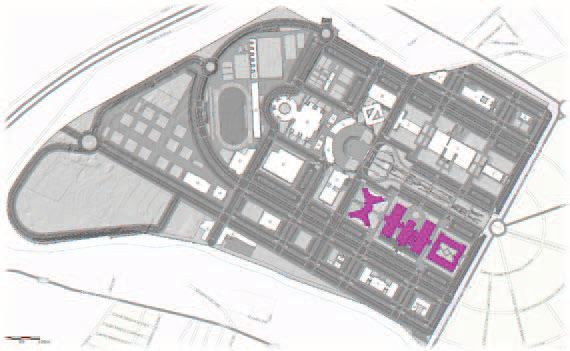
\includegraphics[width=.3\textwidth]{image/uj1.png}\hfill
%     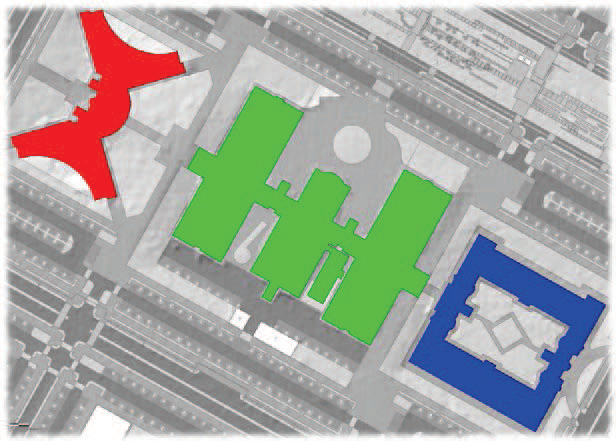
\includegraphics[width=.3\textwidth]{image/uj2.png}\hfill
%     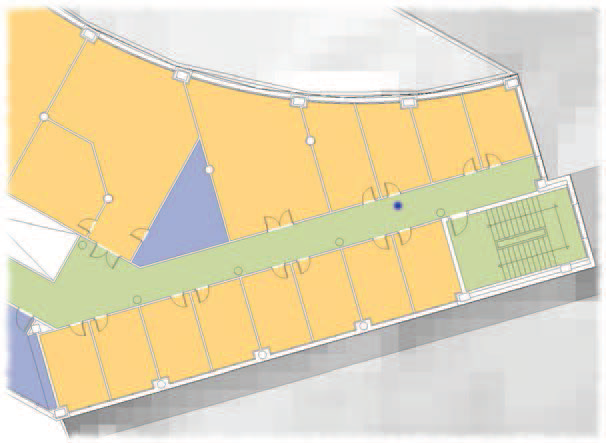
\includegraphics[width=.3\textwidth]{image/uj3.png}
%     \\[\smallskipamount]
%     \caption{Map of the UJI Riu Sec Campus}
%     \label{uji}
% \end{figure}



% \begin{table}[!h]
%     \centering
%     \caption{ Sample information related to  PhoneID and real device. }
%     \label{phone}
%     \begin{tabular}{c c c c}
%     \hline
%      PhoneID & Android Device  & Android Version & UserID \\
%      \hline
%       0 &  Celkon A27  & 4.04 & 0\\
%      \hline
%       1 & GT-I8160   & 2.3.6 &8\\
%      \hline
%       2  &  GT-I8160 & 4.1.2 &0\\
%      \hline
%       3 & GT-I9100   & 4.0.4 &5\\
%      \hline
%       4  & GT-I9300  & 4.1.2 &0\\
%      \hline
%       5  & GT-I9505  & 4.2.2 & 0\\
%      \hline
%       6 & GT-S5360  &2.3.6  & 7\\
%      \hline
%       7 & GT-S6500  &2.3.6  &14\\
%      \hline
%       8 &  Galaxy Nexus  & 4.2.2  &10\\
%       \hline
%       9 &   Galaxy Nexus & 4.3 &0\\
%      \hline
%       10  & HTC Desire HD  &2.3.5 &0,11\\
%      \hline
%       11  & HTC One  & 4.1.2  & 0,1,9,16\\
%      \hline
%       12 &  HTC One & 4.2.2  & 3\\
%      \hline
%       13 &  HTC Wildfire S &2.3.5  &3\\
%      \hline
%       14 &  LT22i  & 4.0.4  &13\\
%       \hline
%       ... & ...   & ...  &...\\
%       \hline
%       24 & bq Curie   &  4.1.1 & 12\\
%       \hline
%     \end{tabular}
    
% \end{table}


The data was collected From May 30 to June 20, 2013 as shown in Table \ref{udate}. The number of data points show the distribution of measurements during each day. The data collection happened on these six discrete days. The day when the most amount of data was collected was the $20^{th}$ of June. This single day accounts for more than half the points in the entire data set.
%Two Android applications have been used to create the database by applying reference map services that are published in the ArcGIS. These services include geographic information inside the building. By using these services, the applications created show the maps to improve the user localization.


% all dataset capture in 6 days 30,31,may 4,10,12,20June, 19 , 20, 24,26 sep, 1,3,4,7,8 oct
\begin{table}[ht]
\centering
\caption{UJIIndoorLoc Experiment timeline.}
\begin{tabular}{lclc}
\toprule
\textbf{Date} &  \textbf{Number of data points}       \\
\midrule
     \rowcolor{cyan}
5/30/2019                 &      1140                 \\
     \rowcolor{cyan}
5/31/2019                 &      362                  \\
     \rowcolor{cyan}
6/4/2019                  &      1010                 \\
     \rowcolor{cyan}
6/10/2019                 &      270                 \\
     \rowcolor{cyan}
6/12/2019                 &      2467                 \\
     \rowcolor{cyan}
6/20/2019                 &      14688                \\
\bottomrule
\label{udate}
\end{tabular}
\end{table}



% \begin{enumerate}
%     \item\textbf{RSSI Levels:} These values show the RSSI levels by  WAP identifiers (MAC addresses) are linked to the vector positions. The RSSI levels represent negative integer values measured in dBm. In this measure, −100dBm is equivalent to the weak signal, and 0dBM indicates that the detected WAP is a very good signal. The value +100dBm in WAPs records shows that the signal has not been detected by the device.
%     \item\textbf{Real world coordinates:} It means three value, the longitude and latitude coordinates and the floor of the building. 
%     \item\textbf{Space identifier:} Is the value from 0 to 2 and corresponds the building campus. As figure \ref{uji} shows the UJI university campus
%     \item\textbf{User identifier:} This column ranges between 1 to 18 which 18 users are participated to gather the data. 
%     \item\textbf{Phone identifier:} It shows the android device used for this experiment. Table \ref{phone} shows the correspondence between each Phone ID and device used. The device's information included model and android version.
%     \item\textbf{Timestamp:} The time of when signal strength captured in Unix time format is available in the last column. This time is different with each phone time.
    
% \end{enumerate}



% \item\textbf{Data Pre-processing:}
A set of pre-processing tasks were performed to improve the quality of the data set and make the measurements suitable for cluster analysis.
%with the project scope and removed from the dataset.
The timestamp was recorded in a Linux-based time format, such as 1371714467, which corresponds to \texttt{06/20/2013 at 7:47 am}. All the time values were converted to the standard date-time format (dd/mm/yy hh:mm:ss) in Python and added as a new feature called Datetime into the data set.

The feature Space ID contains values starting from 1 to 250, but there were gaps between numbers 50-100 and 150-200. These gaps were removed, and the updated Space ID numbers range from 1 to 122.
These space ID values were not unique in terms of spaces such as offices, classrooms, and labs. 
The Space ID, Building ID, Floor, and relative position together provide a unique label for a location. A new feature is added to the data set called SPACEID, that contains a unique spatial identifier for each location. The SPACEID was created by combining the space identifiers and then giving them a sequential numbers from 0-732.

During the six days of collecting data, some phones (Phone ID = 0,2,4,5,9,12,15,20, and 21) were not used. To make it consecutive, gaps removed and a new feature called PHONEID added to the data with numbers between 1 to 16 for all presented phones.
Table \ref{phone} shows the phone ID related to each android device, the version of the operating system and finally, which user uses the phone. A total of 18 users with sixteen different phones are used for this research. The phone number 9 shared between three users with numbers 1, 9, and 16.




 

\begin{table}[!ht]
    \centering
    \caption{ Correspondence between PhoneID, real device and userID. }
    \label{phone}
    \begin{tabular}{c c c c}
    \hline
     \textbf{PhoneID} & \textbf{Android Device}  & \textbf{Android Version} & \textbf{UserID} \\
     \hline\midrule
      1 & GT-I8160   & 2.3.6 &8\\
     \hline
      2 & GT-I9100   & 4.0.4 &5\\
     \hline
      3 & GT-S5360  &2.3.6  & 7\\
     \hline
      4 & GT-S6500  &2.3.6  &14\\
     \hline
      5 &  Galaxy Nexus  & 4.2.2  &10\\
      \hline
      6  & HTC Desire HD  &2.3.5 &18\\
     \hline
      7  & HTC One  & 4.1.2  & 15\\
     \hline
      8 &  HTC Wildfire S &2.3.5  &11 \\
     \hline
      9 &  LT22i  & 4.0.4  &1,9,16\\
     \hline
      10 &  LT26i  & 4.0.4  &3\\
      \hline      
      11 &  M1005D  & 4.0.4  &13\\
      \hline
      12 &  MT11i  & 2.3.4  &4\\
      \hline      
      13 &  Nexus 4 & 4.2.2  &6\\
      \hline     
      14 &  Orange Monte Carlo  & 2.3.5  &17\\
      \hline      
      15 &  Transformer TF101  & 4.0.3  &2\\
      \hline
      16 & bq Curie   &  4.1.1 & 12\\
      \hline\midrule
    \end{tabular}
    
\end{table}





% Two numerical variables were selected: the SPACEID and the Phone ID for this study as these provide the necessary information regarding the people present at any location with time. Finally, in order to remove bias due to the difference in range of the two variables the data was normalized. The normalization process is applied one level before clustering with the minmaxscaler normalization process under the preprocessing library. All these preceding steps provide a target data set ready to be used by the stream simulation and the two-phase clustering algorithms. 

For cluster analysis, The days are non-uniformly distributed over 2 month as shown in Table \ref{udate} earlier. The data collection during those six days was not continuous but collected at a much higher cadence. A small landmark time window of 10 minutes was applied on this dataset. Moreover, The hyperparameters for the AP in the DSAP algorithm are consistent and fixed for the entire experiment. The damping value is equal to 0.9, maximum iteration is 100, and preference is equal to the median of the similarity matrix. 

Finally, the variable selection task was performed to prepare a target data set ready to be used by the two phase clustering algorithm. For this research, two numerical variables as summarised in Table \ref{select2}.


\begin{table}[!ht]
\centering
\caption{Selected input variables for clustering the data points}
\label{select2}
\begin{tabular}{
>{\columncolor[HTML]{FFFFFF}}c cc}
\hline
\textbf{Variable}              & \cellcolor[HTML]{FFFFFF}\textbf{Description}                                                          & \textbf{Values}     \\ \hline
{\color[HTML]{000000} PHONEID} & {\color[HTML]{000000} \begin{tabular}[c]{@{}c@{}}Each phone represents a\\  participant\end{tabular}} & Range between 1 -16 \\ \hline
{\color[HTML]{000000} SPACEID} & {\color[HTML]{000000} \begin{tabular}[c]{@{}c@{}}Each space represents a \\ location\end{tabular}}    & Range between 0-732 \\ \hline
\end{tabular}
\end{table}


% \begin{itemize}
%     \item A constant damping factor equal to 0.9 for AP algorithm.
%     \item The maximum iteration for AP is the predefined value and it is equal to 100.
%     \item The preference hyper-parameter for AP is the median value of the similarity matrix.
%     \item The expiration value equal to the last 5 landmark window is chosen. 
%     \item The time frame for this data is every 10 minutes.

    
% \end{itemize}


%\item\textbf{Data Stream Simulation:}
%In the simulation phase, we employed two techniques for our model as mentioned before for the for the e-counter data. These techniques are Scikit-Multiflow-based simulation for the DSAP algorithm in Python programming language and DSD-based simulation for the streaming K-means implements in R programming language. These methods are easy to use and can handle live stream from .CSV file. The input of this phase is UJIIndoorLoc dataset for generating the stream simulation and illustrated in Table\ref{ssiimm}. Scikit-Multiflow uses \textit{'skmultiflow.data.FileStream'} simulation class for batch dataset, and DSD used \textit{'stream'} package to implement the stream. 

% \begin{itemize}
%     \item \textbf{Scikit-Multiflow-based Simulations:}
%     \item \textbf{DSD-based Simulations:}
% \end{itemize}

% \begin{table}[!h]{}
% \centering
% \caption{The input data for stream simulation phase.}
% \begin{tabular}{lclcl}
% \toprule
% \textbf{Timestamp} & \textbf{SpaceID } & \textbf{PhoneID}    \\
% \midrule
% 5/30/2013 10:15:24             &   102    &     13       \\
% 5/30/2013 10:15:28             &   102    &     13       \\
% 5/30/2013 10:15:31             &   102    &     13       \\
% 5/30/2013 10:15:35             &   102    &     13       \\
% ...                            &   ...    &     ...      \\
% ...                            &   ...    &     ...      \\
% % 10/8/2013 3:56:47              &   0      &     13       \\
% % 10/8/2013 3:57:16              &   0      &     13       \\
% \bottomrule
% \label{ssiimm}
% \end{tabular}
% \end{table}


%\end{itemize}


% \subsubsection{Data Stream Clustering} 
% 




%Processing time is calculated by subtract the end time from starting time with the  $time()$ method. Memory usage obtained from $psutil$ library in Python for processes and system utilization as same as $memory$ in R programming language. Outlier Detection, Processing Time, and Memory Consumption. 

% \hspace{1 cm}

\section{System and Software}

Various tools and languages were used and they are listed below.

\begin{itemize}
    \item\textit{Platform:} This research work was performed on a personal computer running on a 64-bit operating system, window 10 Enterprise, 2019. The specification of this machine are: Intel Core i7 2.60GHz CPU, 32GB internal memory RAM, and 3TB external memory. 
    \item\textit{Language selection:} DSAP is developed in Python. The version of Python used is 3.7. Spyder 3.3.6 IDE which is part of Anaconda 2019 was used for project development. Main libraries applied in Python are sklearn, pandas, numpy, matplotlib, datetime, scipy, psutil and itertools.
    
    %Other programming language used for development and visualization are R and matlab. The versions used are RStudio 1.2.5033, 2019 and matlab 2019. 
    
    \item\textit{Software:} Microsoft Excel 2020 was used for preliminary visualization of the .CSV file format. It has a neat feature to quickly filter the data and visualize.
    
    Lucidchart web-based platform is another software that was used for drawing, revising and sharing charts and diagrams.
    

\end{itemize}

% some lat lang 2 user capture the poin t the same time with diffrent phones

% \end{document}


%%%%%%%%%%%%%%%%%%%%%%%%%%%%%%%%%%%%%%%%%%%%%%%%%%%%%%%%%%%%%%%%%%%%%%%%%%%%%%%%%%%%%%%%%%%%%%%%

% \section{Occupant Behaviour Experiment }\label{wifidat}


% This case study was carried out to find occupant  behavior patterns  in  indoor  spaces  to provide  relevant  information  for  future planning  building  automation, evaluating energy efficiency scenarios, and simulating   emergency   protocols. The experiment was conducted over four months at the Universitat Jaume I campus, in Valencia, Spain. During this time, users carried mobile devices that used \textit{CaptureLoc} to record eight types of attributes including user position and WiFi signal strength across a total of thirteen levels spanning three buildings of the campus. To protect the identity of the participants during the course of the experiment, the unique MAC identifiers of the phones were hashed (anonymized) on reception.


% The UJIIndoorLoc data set generated includes three buildings with four or more floors (one building has five floors) and almost 110.000 m$^{2}$of space. The total number of locations captured was 732. The shape and structure of the three buildings TI, TD, and TC, are quite different, as shown in Figure \ref{dspp2}. The raw data set consists of 19,937 data points containing 529 attributes as illustrated in Table \ref{featuj}. These attributes include the Received signal strength indicator (RSSI) for 520 wireless access points (WAPs). 

% \begin{figure*}[!h]
% \centering
% \subfloat[Overview of the three buildings]{\label{fig:build}{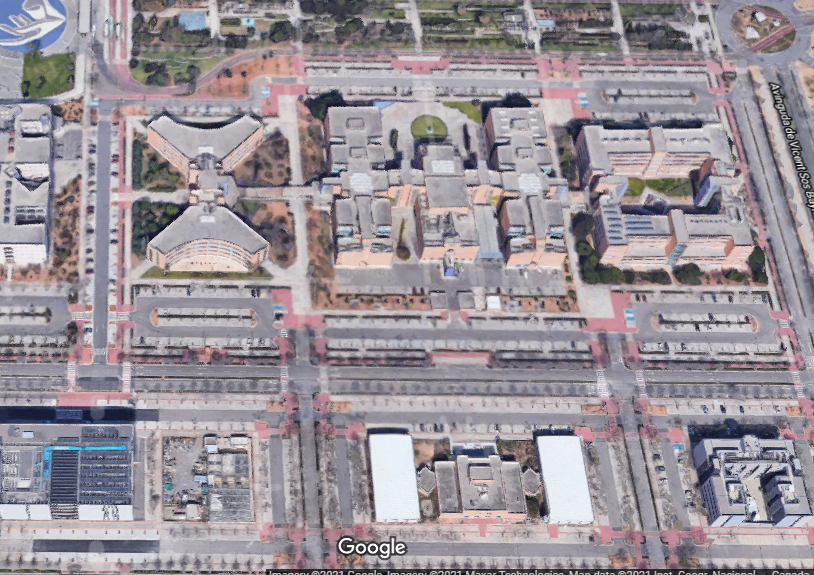
\includegraphics[width=7 cm, height = 6 cm]{image/Chapters/Chapter5/uji.PNG}}}\hfill
% \subfloat[Building Number 0 (TI)]{\label{fig:bl2}{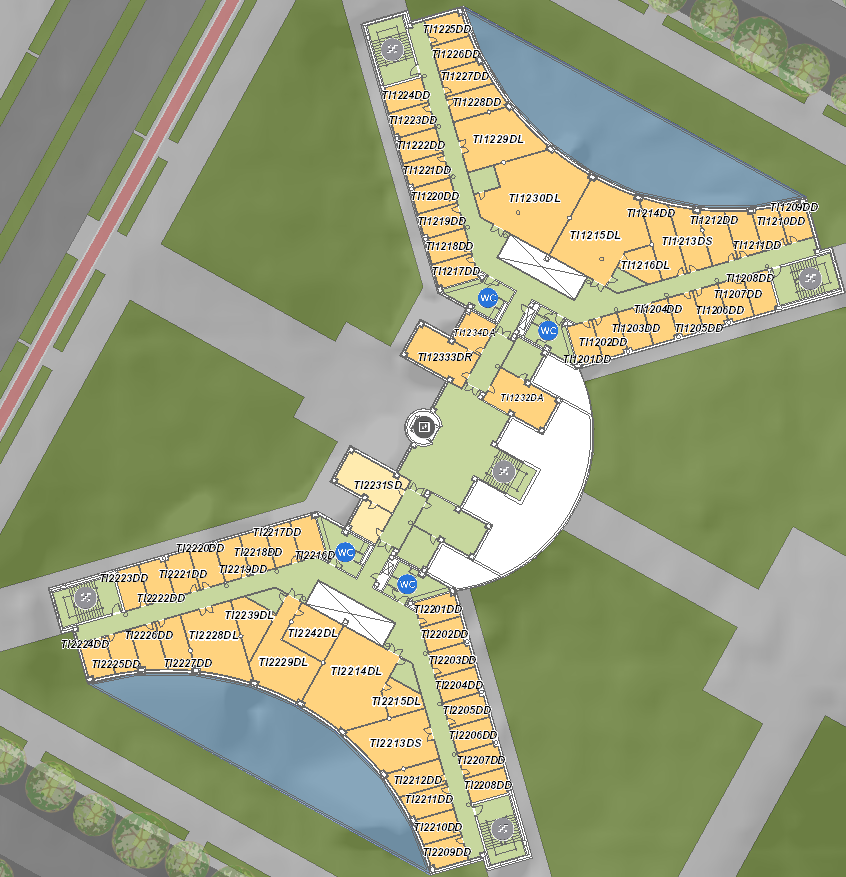
\includegraphics[width=0.4\textwidth]{image/plan2.png}}}\hfill
% \subfloat[Building Number 1 (TD)]{\label{fig:bl3}{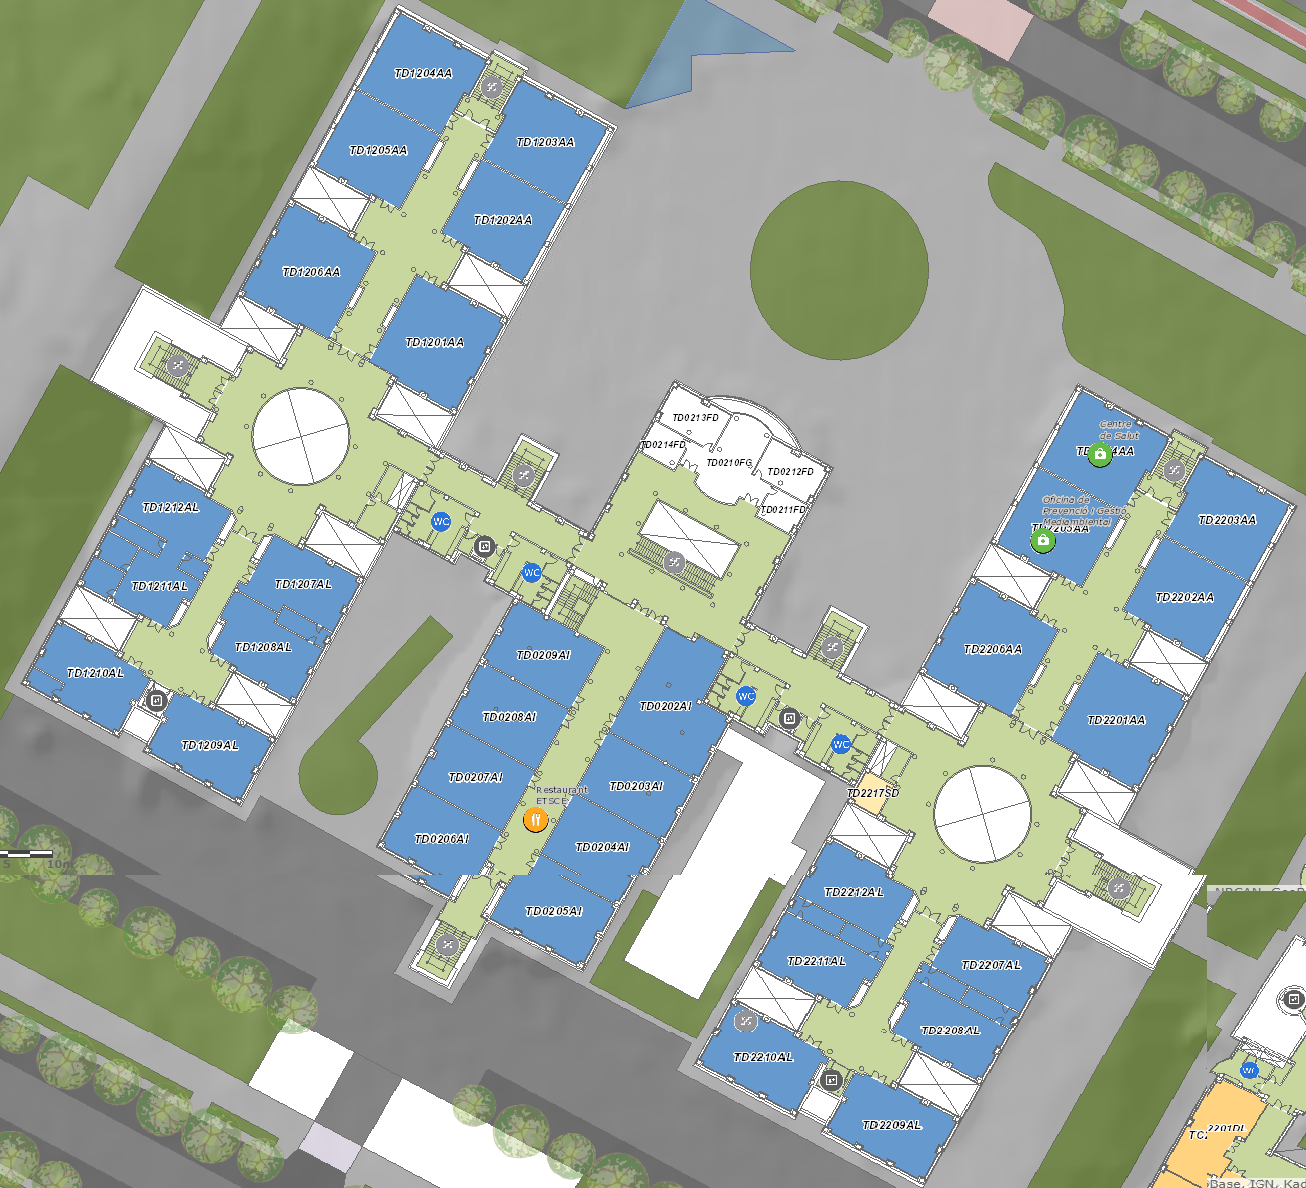
\includegraphics[width=0.4\textwidth]{image/plan3.png}}}\hfill
% \subfloat[Building Number 2 (TC)]{\label{fig:bl4}{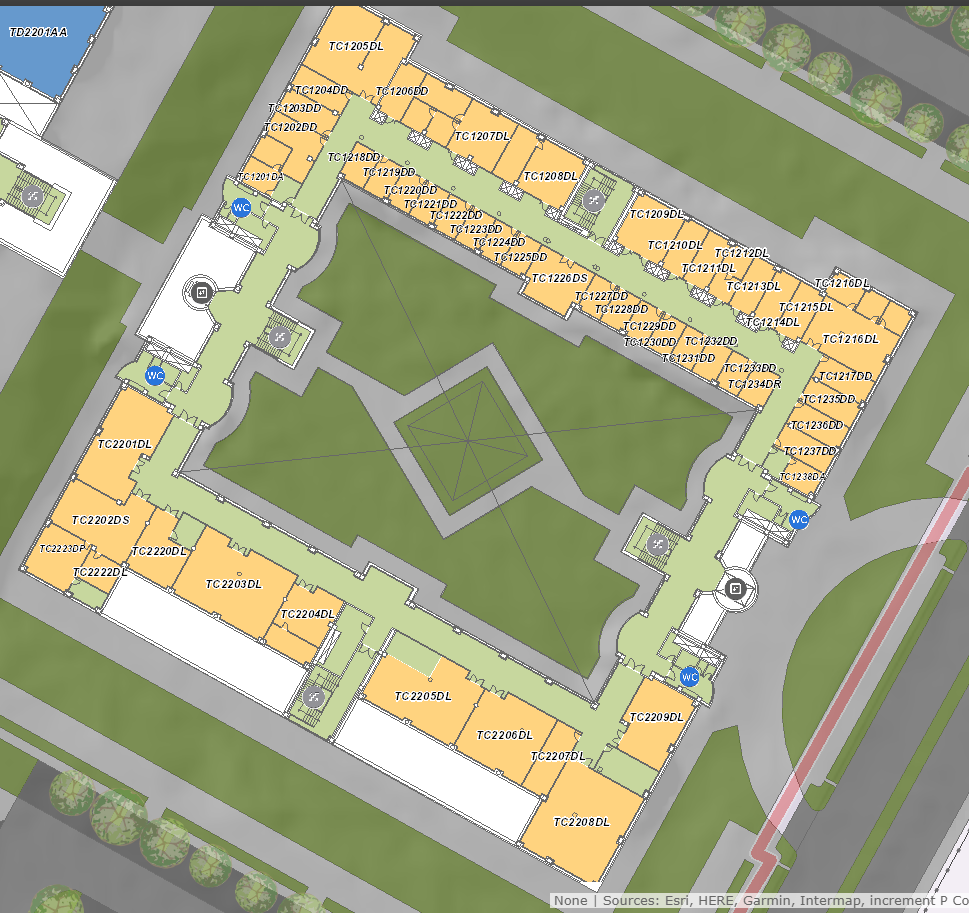
\includegraphics[width=0.4\textwidth]{image/plan1.png}}}\hfill
% \caption{(a) Map of the UJI Riu Sec Campus and the buildings used for WiFi fingerprint experiment. (b,c,d) The layout of the three buildings with spaceid numbers for a floor.}% is shown with purple color. A zoom of T1, TD, and TC building shows. Inside the plans we have information regarding spaceID.}
% \label{dspp2}
% \end{figure*}

% %***** remove 
% \begin{table}[!h]{}
% \centering
% \caption{ List of attributes of the UJIIndoorLoc data set.}
% \small
%     \begin{tabular}{ p{4cm} p{4.5cm} p{4.5cm} }
%     \hline
%     \textbf{Attributes} & \textbf{Measurement} & \textbf{Definition} \\ \hline
%     \midrule
%     RSSI Level             &    -100dBM: weak signal, 0dBM: good, 100dBM: not detected    & RSSI levels where the WAP identifiers are linked to the vector positions           
%     \\\hline
%     Longitude              &    UTM from WGS84     &  Y coordinates           \\\hline
%     Latitude               &    UTM from WGS84     &  X coordinates          \\\hline
%     Floor                  &    0,1,2,3,4     &  Floors of each building           
%     \\\hline
%     Building ID            &    0,1,2     &  Each of the three buildings TI,TD, and TC          
%     \\\hline
%     Space ID               &    integer   & Identification of an indoor space (e.g. room or corridor)            
%     \\\hline
%     Relative Position      &    1= inside 2=outside       & Outside means in front of the door of the space \\\hline
%     User ID                &    1,2,...,18    &  Unique code for users who participated in the experiment           \\\hline
%     Phone ID               &    1,2,...,16      &    Android device code used for this experiment        \\\hline
%     Timestamp              &    Unix time format      &  Time of capture           
%     \\
%     \bottomrule
% \label{featuj}
% \end{tabular}
% \end{table}


% A total of 18 users with sixteen different phones participated in the study as listed in Table \ref{phone}. This table show the phone ID related to each android device, the version of the operating system and finally, which user uses the phone. The phone number 9 shared between three users with numbers 1, 9, and 16. 

% \begin{table}[!h]
%     \centering
%     \caption{ Sample information related to  PhoneID and real device. }
%     \label{phone}
%     \begin{tabular}{c c c c}
%     \hline
%      \textbf{PhoneID} & \textbf{Android Device}  & \textbf{Android Version} & \textbf{UserID} \\
%      \hline\midrule
%       1 & GT-I8160   & 2.3.6 &8\\
%      \hline
%       2 & GT-I9100   & 4.0.4 &5\\
%      \hline
%       3 & GT-S5360  &2.3.6  & 7\\
%      \hline
%       4 & GT-S6500  &2.3.6  &14\\
%      \hline
%       5 &  Galaxy Nexus  & 4.2.2  &10\\
%       \hline
%       6  & HTC Desire HD  &2.3.5 &18\\
%      \hline
%       7  & HTC One  & 4.1.2  & 15\\
%      \hline
%       8 &  HTC Wildfire S &2.3.5  &11 \\
%      \hline
%       9 &  LT22i  & 4.0.4  &1,9,16\\
%      \hline
%       10 &  LT26i  & 4.0.4  &3\\
%       \hline      
%       11 &  M1005D  & 4.0.4  &13\\
%       \hline
%       12 &  MT11i  & 2.3.4  &4\\
%       \hline      
%       13 &  Nexus 4 & 4.2.2  &6\\
%       \hline     
%       14 &  Orange Monte Carlo  & 2.3.5  &17\\
%       \hline      
%       15 &  Transformer TF101  & 4.0.3  &2\\
%       \hline
%       16 & bq Curie   &  4.1.1 & 12\\
%       \hline\midrule
%     \end{tabular}
    
% \end{table}


% % \begin{table}[!h]
% %     \centering
% %     \caption{ Sample information related to  PhoneID and real device. }
% %     \label{phone}
% %     \begin{tabular}{c c c c}
% %     \hline
% %      \textbf{PhoneID} & \textbf{Android Device}  & \textbf{Android Version} & \textbf{UserID} \\
% %      \hline\midrule
% %       1 & GT-I8160   & 2.3.6 &8\\
% %      \hline
% %       3 & GT-I9100   & 4.0.4 &5\\
% %      \hline
% %       6 & GT-S5360  &2.3.6  & 7\\
% %      \hline
% %       7 & GT-S6500  &2.3.6  &14\\
% %      \hline
% %       8 &  Galaxy Nexus  & 4.2.2  &10\\
% %       \hline
% %       10  & HTC Desire HD  &2.3.5 &18\\
% %      \hline
% %       11  & HTC One  & 4.1.2  & 15\\
% %      \hline
% %       13 &  HTC Wildfire S &2.3.5  &11 \\
% %      \hline
% %       15 &  LT22i  & 4.0.4  &1,9,16\\
% %      \hline
% %       16 &  LT26i  & 4.0.4  &3\\
% %       \hline      
% %      \hline
% %       17 &  M1005D  & 4.0.4  &13\\
% %       18 &  MT11i  & 2.3.4  &4\\
% %       \hline      
% %       19 &  Nexus 4 & 4.2.2  &6\\
% %       \hline     
% %       22 &  Orange Monte Carlo  & 2.3.5  &17\\
% %       \hline      
% %       23 &  Transformer TF101  & 4.0.3  &2\\
% %       \hline
% %       24 & bq Curie   &  4.1.1 & 12\\
% %       \hline\midrule
% %     \end{tabular}
    
% % \end{table}


% The data was collected From May to June 2013 as shown in Table \ref{udate}. The number of data points show the distribution of measurements during each day. The data collection happened on 6 discrete days. The day when the most amount of data was collected was the 20th of June. This single day accounts for more than half the points in the entire data set. 
% %Two Android applications have been used to create the database by applying reference map services that are published in the ArcGIS. These services include geographic information inside the building. By using these services, the applications created show the maps to improve the user localization.



% \begin{table}[ht]
% \centering
% \caption{UJIIndoorLoc Experiment timeline.}
% \begin{tabular}{lclc}
% \toprule
% \textbf{Date} &  \textbf{Number of data points}       \\
% \midrule
%      \rowcolor{cyan}
% 5/30/2019                 &      1140                 \\
%      \rowcolor{cyan}
% 5/31/2019                 &      362                  \\
%      \rowcolor{cyan}
% 6/4/2019                  &      1010                 \\
%      \rowcolor{cyan}
% 6/10/2019                 &      270                 \\
%      \rowcolor{cyan}
% 6/12/2019                 &      2467                 \\
%      \rowcolor{cyan}
% 6/20/2019                 &      14688                \\
%      \rowcolor{pink}
% 9/19/2019                 &      51                   \\
%      \rowcolor{pink}
% 9/20/2019                 &      133                  \\
%      \rowcolor{pink}
% 9/24/2019                  &     56                   \\
%      \rowcolor{pink}
% 9/26/2019                  &     69                   \\
%      \rowcolor{pink}
% 10/1/2019                  &     8                    \\
%      \rowcolor{pink}
% 10/3/2019                  &     8                    \\
%      \rowcolor{pink}
% 10/4/2019                  &     702                  \\
%      \rowcolor{pink}
% 10/7/2019                  &     81                   \\
%      \rowcolor{pink}
% 10/8/2019                  &     3                    \\
% \bottomrule
% \label{udate}
% \end{tabular}
% \end{table}



% A set of pre-processing tasks were performed to improve the quality of the data set and make the measurements suitable for cluster analysis.
% %with the project scope and removed from the dataset.
% The timestamp was recorded in a linux-based time format, such as 1371714467 which corresponds to 06/20/2013 at 7:47am. All the time values were converted to the standard date-time format (dd/mm/yy hh:mm:ss) in Python and added as a new feature called Datetime into the data set.

% The feature SpaceID contains values starting from 1 to 250, but there were gaps between numbers 50-100 and 150-200. These gaps were removed and the updated SpaceID numbers range from 1 to 122 now. During the validation part of the experiment a subset of the phones (PhoneID = 0,2,4,5,9,12,15,20, and 21) were not used. The remaining Phoneids were renamed to make the records sequential just like the SpaceIDs. The space identifiers, the SpaceID, BuildingID, Floor, and relative position together provide a unique label for a location. A new feature is added to the data set called SPACEID, that contains a unique spatial identifier for each location. The SPACEID was created by combining the space identifiers and then giving them a sequential numbers from 0-732.

% For cluster analysis, The days are non-uniformly distributed over 2 month as shown in Table \ref{udate} earlier. For the training data, The data collection during those six days was not continuous but collected at a much higher cadence. For these reasons a smaller landmark time window of 10 minutes was applied on this dataset. Moreover, The hyperparameters for the AP in the DSAP algorithm are consistent and fixed for the entire experiment. The damping value is equal to 0.9, maximum iteration is 100, and preference is equal to the median of the similarity matrix.